\documentclass[11pt]{article}
%\documentclass[11pt,dvipdfm]{article} 

\usepackage{deauthor,times,graphicx}
%\usepackage[hidelinks]{hyperref}
\usepackage{tcolorbox}
%\graphicspath{{istvan/}} 
\usepackage{xpatch}
\usepackage{xspace}
\usepackage{multirow}


\makeatletter

\makeatletter

\newcommand{\hi}[1]{\noindent {\bf #1}}

\newcommand{\lgl}[1]{{\textcolor{blue}{{#1}}}}

\newcommand{\oursys}{\textsf{XuanYuan}\xspace}

\begin{document}

%\pagestyle{plain}
%\pagenumbering{arabic}


\setcounter{figure}{0}  

% ****************** AUTHORS **************************************

\title{\oursys: An AI-Native Database}

%\author{Zsolt Istv\'{a}n\\ \small IMDEA Software Institute, Madrid, Spain\\  \small \{first.lastname@imdea.org\}}
\author{Guoliang Li, Xuanhe Zhou, Sihao Li\\ 
\small Department of Computer Science,Tsinghua University, Beijing, China\\
\small Gauss Database Group, Huawei Company\\  
\small liguoliang@tsinghua.edu.cn}

\maketitle

\begin{abstract}
Online crowdsourcing platforms have proliferated over the last few years and cover a number of important domains, these platforms include from worker-task platforms such Amazon Mechanical Turk, worker-for-hire platforms such as TaskRabbit to specialized platforms with specific tasks such as ridesharing like Uber, Lyft, Ola etc.
An increasing proportion of human workforce will be employed by these platforms in the near future.
The crowdsourcing community has done yeoman's work in designing
effective algorithms for various key components, such as incentive design, task assignment and quality control. Given the increasing importance of these crowdsourcing platforms,
it is now time to design mechanisms so that it is easier to evaluate the effectiveness of these platforms. Specifically, we advocate developing benchmarks for crowdsourcing research.

Benchmarks often identify important issues for the community to focus and improve upon.
This has played a key role in the development of research domains as diverse as
databases and deep learning.
We believe that developing appropriate benchmarks for crowdsourcing will ignite further innovations.
However, crowdsourcing -- and future of work, in general -- is a very diverse field
that makes developing benchmarks much more challenging.
Substantial effort is needed that spans across developing benchmarks for
datasets, metrics, algorithms, platforms and so on.
In this article, we initiate some discussion into this important problem and
issue a call-to-arms for the community to work on this important initiative.
\end{abstract}

\section{Introduction}
\label{sec:intro}

Federated Learning (FL) is a distributed machine learning (ML) paradigm that trains a model across a number of participating entities holding local data samples.
% , without exchanging them. 
In this work, we focus on \emph{cross-device} FL that harnesses a large number (up to hundreds of millions) of edge devices with disparate characteristics such as availability, compute, memory, or connectivity
resources~\citep{kairouz2019advances}. %that harnesses potential
% Current applications of FL are designed to scale up to client populations of hundreds of millions or even billions. 
Two challenges to the success of cross-device FL are privacy and scalability. 
FL was originally motivated for improving privacy since data points remain on client devices. 
% and only small model updates were shared to a co-ordinating server.
However, as with other forms of ML, information about training data can be extracted via membership inference or reconstruction attacks on a trained model \citep{carlini2021membership,carlini2020extracting}, or leaked through local updates~\citep{MelisSCS19,geiping2020inverting}. 
Consequently, Secure Aggregation (\SecAgg) protocols were introduced to prevent the server from directly observing individual client updates, which is a major vector for information leakage~\citep{bonavitz2019federated,huba2021papaya}. 
Additional mitigations such as  Differential Privacy (DP) may be required to offer further protection 
against attacks~\citep{dwork2006calibrating,abadi2016deep}, as discussed in Section~\ref{sec:discussion}.
% , as discussed in Section~\ref{sec:discussion}.
%As an additional layer of protection against statistical inference attacks, SecAgg is usually paired with Differential Privacy (DP) \citep{dwork2006calibrating}. To realize the full promise of FL as a privacy-enhancing technology, we need both SecAgg and Differential Privacy.

Ensuring scalability to populations of heterogeneous clients is the second challenge for FL.
% There are many aspects for FL scalability, such as ensuring that model updates can be calculated efficiently 
% by devices with various capabilities and intermittent availability~\citep{bonavitz2019federated}.
% Here, we focus on the communication bottleneck as the primary concern.
Indeed, wall-clock training times are highly correlated with increasing model and batch sizes~\citep{huba2021papaya}, even with recent efforts such as FedBuff~\citep{nguyen2021federated},
% With increasing model and batch sizes, the wall-clock training time increases accordingly~\citep{huba2021papaya}. 
% Despite efforts such as buffered asynchronous aggregation~\cite{nguyen2021federated}, 
and communication overhead between the server and clients dominates model convergence time.
% cross-device FL remains bottlenecked by communication latency between the server and the clients. 
% \karthik{should we mention this paper in a different way? Fedbuff paper doesn't explicitly call out latency as an issue, nor do we run experiments to on async fl ourselves}  \ashkan{I also think the transition can be smoother: first we focus on scalability and billions. Then we say communication is the bottleneck} 
Consequently, compression techniques were used to reduce the communication bandwidth while maintaining model accuracy.
However, a fundamental problem has been largely overlooked in the literature: in their native form, standard compression methods such as scalar quantization and pruning are not compatible with \SecAgg. 
This makes it challenging to ensure both security and communication efficiency.
% at the same time.
% the default method to provide security for client update, 
% presenting an unpleasant dichotomy between security or efficiency. 


% Second, this is the most restricted direction, since upload bandwidth remains more restricted than download. 
% In the US, fixed-line broadband speeds typically achieve a ratio of $3\times$ to $20\times$ more download bandwidth than upload
% bottlenecks remain, and so we seek to reduce the message size of clients by \textit{compression}. 
% Compression has been widely proposed in various ML scenarios, in the form of pruning (removing model parameters) and quantization (reducing fidelity of parameter representation). 
% Indeed, these techniques have been successfully used in FL settings with appreciable improvements in communication while maintaining model accuracy. 
% However, there is a fundamental problem which has been largely overlooked in the literature: in their native form, these compression methods are not compatible with SecAgg, the default method to provide security for client updates. 
% This presents an unpleasant dichotomy: we can have security or efficiency, but not both. 
%
%
% In this paper, we resolve this gap by showing how to modify FL compression techniques to make them security-friendly. We focus on compressing \emph{uplink} updates from clients to the server for two reasons. 
% First, uplink communications are subject to Secure Aggregation protocols to ensure a high security bar, while downlink updates broadcasted by the server are deemed public. 
% Second, upload bandwidth is generally more restricted than download. For instance, according to the most recent FCC report, the ratio of download to upload speeds for DSL/cable providers\footnote{Fixed-line broadband is most relevant since FL is typically restricted to using unmetered connections, usually over Wi-Fi~\citep{huba2021papaya}.} in the US ranges between 3$\times$ to 20$\times$~\citep{fcc-broadband}.
% % This requires some meticulous changes to coordinate clients to use the same global (non-private) hyperparameters, and show that this coordination does not damage model quality. 
% % For the strongest compression methods, we step outside of the SecAgg primitive and propose a new secure primitive, Secure Indexing, which enables the best compression ratios without sacrificing utility. 
% Finally, efficient and secure uplink communication brings several benefits beyond speeding up convergence: 
% lowering communication cost reduces selection bias due to undersampling clients with limited connectivity, improving fairness and inclusivity metrics. 
% It also shrinks the carbon footprint of FL, whose fraction attributable to communication can reach 95\%~\citep{qiu2021first}.
%
%In this paper, w
We address this gap by adapting compression techniques to make them compatible with \SecAgg. We focus on compressing \emph{uplink} updates from clients to the server for three reasons. 
First, uplink communication is more sensitive and so is subject to a high security bar, whereas downlink updates broadcast by the server are deemed public. 
Second, upload bandwidth is generally more restricted than download bandwidth. For instance, according to 
a recent FCC report, 
%the most recent \modif{FCC\footnote{\modif{US Federal Communications Commission.}} report}, 
the ratio of download to upload speeds for DSL and cable providers\footnote{FL is typically restricted to using unmetered connections, usually over Wi-Fi~\citep{huba2021papaya}.} in the US ranges between 3$\times$ to~20$\times$~\citep{fcc-broadband}.
% Fixed-line broadband is most relevant since
% This requires some meticulous changes to coordinate clients to use the same global (non-private) hyperparameters, and show that this coordination does not damage model quality. 
% For the strongest compression methods, we step outside of the SecAgg primitive and propose a new secure primitive, Secure Indexing, which enables the best compression ratios without sacrificing utility. 
Efficient uplink communication brings several benefits beyond speeding up convergence: 
lowering communication cost reduces selection bias due to under-sampling clients with limited connectivity, improving fairness and inclusiveness. 
It shrinks the carbon footprint of FL, the fraction of which attributable to communication can reach 95\%~\citep{qiu2021first}.
In summary, we present the following contributions: 
\begin{itemize}
    \item We highlight the fundamental mismatch between two critical components of the FL stack: \SecAgg protocols and uplink compression mechanisms.
    
    \item We formulate solutions by imposing a linearity constraint on the decompression operator, as illustrated in Figure~\ref{fig:secagg_summary} in the case of TEE-based \SecAgg.
    
    \item We adapt the popular scalar quantization and (random) pruning compression methods for compatibility with the FL stack that require no changes to the \SecAgg protocol.
    
    \item For extreme uplink compression without compromising security, we propose Secure Indexing (\SecInd), a variant of \SecAgg that supports product quantization. %and admits a secure implementation.
\end{itemize}

\begin{figure*}[t]
    \centering
    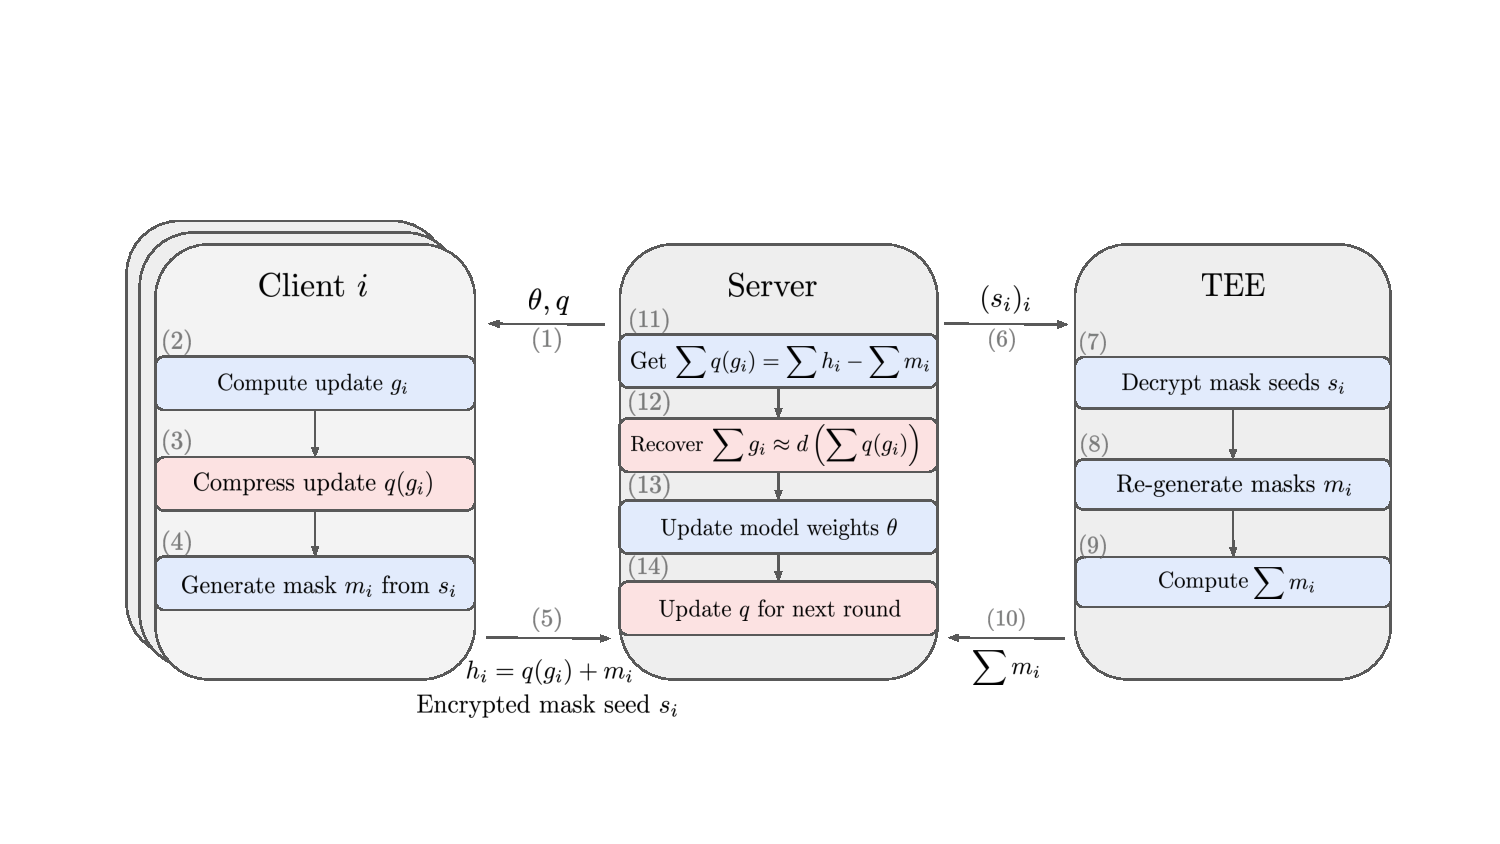
\includegraphics[width=0.8\textwidth]{figs/secagg_summary_new.pdf}
    %\vspace{-5mm}
    \caption{\label{fig:secagg_summary}
    Summary of the proposed approach for one FL round, where we omit the round dependency and \modif{Differential Privacy (DP)} for clarity. Blue boxes denote standard steps and red boxes denote additional steps for uplink compression. Client $i$ computes local model update $g_i$, compresses it with the compression operator $q$, and encrypts it by adding a random mask $m_i$ in the compressed domain, hence reducing the uplink bandwidth (steps 2--4). The server recovers the aggregate in the compressed domain by leveraging any \SecAgg protocol \modif{(steps 7--13, with a TEE-based \SecAgg, see Section~\ref{subsec:secagg})}. Since the decompression operator $d$ is linear, the server can convert the aggregate back to the non-compressed domain, up to compression error (step 12). As with the model weights $\theta$, the compression operator $q$ are also periodically updated and broadcast by the server (step 14). 
    In Section~\ref{sec:method}, we apply the proposed method to scalar quantization and pruning without impacting \SecAgg and propose Secure Indexing, a variant of \SecAgg for extreme uplink compression with product quantization. See Section~\ref{subsec:secagg} for details about \SecAgg and Section~\ref{sec:discussion} for a discussion on~DP.
    }
    \vspace{-3mm}
\end{figure*}



% Our focus in this paper is on 

%Second, scaling cross-device (synchronous) FL to millions of clients with various capabilities and intermittent availability \citep{bonavitz2019federated} suffers from diminishing returns: the wall-clock training time plateaus as the number of clients keeps increasing~\citep{huba2021papaya}. Even though this challenge can be addressed by leveraging the buffered asynchronous aggregation technique proposed by \cite{nguyen2021federated}, compatible with DP and SecAgg, the asynchronous protocol remains bottlenecked by communication latency between the server and the clients.


%Considering the above privacy and scalability goals, we focus on enabling efficient FL communications while keeping a high privacy bar. In addition to the primary objective of speeding up convergence, reducing communication costs brings other significant benefits. Lowering communication requirements addresses selection bias due to undersampling clients with limited connectivity, improving fairness and inclusivity metrics. Better communication efficiency shrinks the carbon footprint of FL, whose fraction attributable to communication can reach 95\%~\citep{qiu2021first}. %Finally, training larger model in FL would be a possibility, when the communication cost is reduced, because local memory or compute requirements can be addressed by modifying the local training loop, for instance with gradient checkpointing \citep{chen2016training}. However, some form of compression would be required to enable efficient communication.


%First, compressing model updates from the client to the server presents several challenges due to compatibility with SecAgg and is an area suitable for further research. 
%Second, upload bandwidth is generally more restricted than download. For instance, according to the most recent FCC report, the ratio of download to upload speeds for DSL/cable providers in the US ranges between 3$\times$ to 20$\times$~\citep{fcc-broadband}. We consider broadband speeds here because devices participate in the FL training while connected to fixed broadband, usually through Wi-Fi~\citep{huba2021papaya}.




% Hence, FL provides the ability to leverage data from massive client populations while ensuring the security and privacy of the client data.
% Go further: compatibility with DP / compression as a mitigation techniques of attacks
% Model and gradient compression intrinsically different.
%  Why not having the secure enclave perform the aggregation?

%\newcommand{\parai}[1]{\noindent\textit{#1}}

\section{Background}
\label{sec:background}

In this section, we recall the \SecAgg protocol first, then the compression methods that we wish to adapt to \SecAgg, namely, scalar quantization, pruning, and product quantization.

\subsection{Secure Aggregation}
\label{subsec:secagg}

\SecAgg refers to a class of protocols that allow the server to aggregate client updates without accessing them individually. While \SecAgg alone does not entirely prevent client data leakage, it is a powerful and widely-used component of current at-scale cross-device FL implementations~\citep{kairouz2019advances}. Two main approaches exist in practice: software-based protocols relying on Multiparty Computation (MPC)~\citep{bonavitz2019federated,bell2020secure,LightSecAgg}, and those that leverage hardware implementations of Trusted Execution Environments (TEEs)~\citep{huba2021papaya}. 
% While these approaches have substantial differences, they impose similar constraints on compatible update compression techniques: operating over finite fields and assuming that aggregation commutes with decompression.


\SecAgg relies on additive masking, where clients protect their model updates $g_i$ by adding a uniform random mask $m_i$ to it, guaranteeing that each client’s masked update is statistically indistinguishable from any other value. 
% Masks are generated so that when all the masked client updates are aggregated by the server (typically through addition), the server obtains the exact aggregate (e.g., the sum of updates). 
At aggregation time, the protocol ensures that all the masks are canceled out. For instance, in an MPC-based \SecAgg, the pairwise masks cancel out within the aggregation itself, since for every pair of users $i$ and $j$, after they agree on a matched pair of input perturbations, the masks $m_{i,j}$ and $m_{j,i}$ are constructed so that $m_{i,j}=-m_{j,i}$.
Similarly and as illustrated in Fig.~\ref{fig:secagg_summary}, in a TEE-based \SecAgg, the server receives $h_i = g_i + m_i$ from each client as well as the sum of the masks $\sum_i m_i$ from the TEE and recovers the sum of the updates as
% by unmasking the aggregated updates as 
%\begin{equation*}
$
      \sum_i g_i = \sum_i h_i - \sum_i m_i.
$
%\end{equation*}
We defer the discussion of DP noise addition by \SecAgg protocols to Section~\ref{sec:discussion}.

\para{Finite Group.}
\SecAgg requires that the plaintexts---client model updates---be elements of a finite group, while the inputs are real-valued vectors represented with floating-point types. 
This requirement is usually addressed by converting client updates to fixed-point integers and operating in a finite domain (modulo~$2^p$) where $p$ is typically set in prior literature to 32 bits. The choice of \SecAgg bit-width~$p$ must balance communication costs with the accuracy loss due to rounding and overflows.

% The other constraint is due to the fact that SecAgg is designed so that the server sees only the aggregate (the sum or the weighted sum) of individual gradients, plus some noise injected by a differentially private mechanism. A drop-in decompression operator $D$ must commute with SecAgg, or be close to being one:
% \[
% D\left(\sum_i g_i+\mathrm{noise}\right) \approx \sum_i D(g_i)+\mathrm{noise}. 
% \]
\para{Minimal Complexity.}
\looseness=-1
TEE-based protocols offer greater flexibility in how individual client updates can be processed; however, the code executed inside TEE is part of the trusted computing base (TCB) for all clients. In particular, it means that this code must be stable, auditable, defects- and side-channel-free, which severely limits its complexity. Hence, in practice, we prefer compression techniques that are either oblivious to \SecAgg's implementation or require minimal changes to the TCB.

% In the remainder of the paper, we focus on the TEE-based approach for its simplicity, scalability and compatibility with asynchronous FL. relies on random masking to encrypt the local model updates. The server then incrementally aggregates the encrypted updates and unmasks the aggregate using the sum of the random masks transmitted by the Trusted Secure Aggregator (TSA) that sits within the TEE. More formally, let us denote $??$ a local client update, represented in floating-point precision, generally \texttt{fp32}. First, the client converts $??$ to a fixed point representation. Then, the client generates a random mask $m \in \Z^d$ and computes the sum modulo a number. \ashkan{TODO}

% SecAgg protocols prevent the server from accessing individual client updates by aggregating them and transmitting only the aggregate to the server. While such mechanisms alone do not entirely prevent data leakage, they constitute a vital component of cross-device FL implementations~\citep{kairouz2019advances}. SecAgg relies either on Secure Multiparty Computation \cite{bonavitz2019federated,so2021secure} or on a Trusted Executed Environment or TEE~\citep{huba2021papaya}. In the remainder of the paper, we focus on the TEE-based approach for its simplicity, scalability and compatibility with asynchronous FL.

% TEE-based SecAgg relies on random masking to encrypt the local model updates. The server then incrementally aggregates the encrypted updates and unmasks the aggregate using the sum of the random masks transmitted by the Trusted Secure Aggregator (TSA) that sits within the TEE. More formally, let us denote $??$ a local client update, represented in floating-point precision, generally \texttt{fp32}. First, the client converts $??$ to a fixed point representation. Then, the client generates a random mask $m \in \Z^d$ and computes the sum modulo a number.

% Since the server, by design, never observes 

\subsection{Compression Methods}
\label{subsec:comp_methods}
In this subsection, we consider a matrix $W \in \mathbb{R}^{\cin\times \cout}$ representing the weights of a linear layer to discuss three major compression methods with distinct compression/accuracy tradeoffs and identify the challenges \SecAgg faces to be readily amenable to these popular quantization algorithms.

\subsubsection{Scalar Quantization}
\label{subsec:sq}

\looseness=-1 Uniform scalar quantization maps floating-point weight $w$ to $2^b$ evenly spaced bins, where $b$ is the number of bits. Given a floating-point scale $s > 0$ and an integer shift parameter $z$ called the zero-point, we map any floating-point parameter $w$ to its nearest bin indexed by $\{0,\dots, 2^b-1\}$:

\centerline{$w \mapsto \clamp(\round(w /s) + z, [0, 2^b - 1] ).$}

%
The tuple $(s, z)$ is often referred to as the quantization parameters (\texttt{qparams}).
With $b=8$, we recover the popular \texttt{int8} quantization scheme \citep{jacob2017quantization}, while setting $b = 1$ yields the extreme case of binarization \citep{courbariaux2015binaryconnect}. 
The quantization parameters $s$ and $z$ are usually calibrated after training a model with floating-point weights using the minimum and maximum values of each layer. 
% The accuracy drop due to this post-training quantization can be mitigated by pre-conditioning the network during training with techniques such as Quantization-Aware Training or QAT~\citep{krishnamoorthi2018quantizing}. 
% The quantization parameters can also be defined per-channel instead of per-layer to diminish the quantization error at the cost of a small memory overhead.
The compressed representation of weights $W$ consists of the \texttt{qparams} and the integer representation matrix $W_q$ where each entry is stored in~$b$~bits. 
Decompressing any integer entry $w_q$ of~$W_q$ back to floating point is performed by applying  the (linear) operator $w_q \mapsto s\times(w_q - z)$.

\para{Challenge.} 
The discrete domain of quantized values and the finite group required by \SecAgg are not natively compatible because of the overflows that may occur at aggregation time. For instance, consider the extreme case of binary quantization, where each value is replaced by a bit. 
We can represent these bits in \SecAgg with $p=1$, but the aggregation will inevitably result in overflows.

\subsubsection{Pruning}
\label{subsec:rp}

Pruning is a class of methods that remove parts of a model such as connections or neurons according to some pruning criterion, such as weight magnitude~(\cite{lecun1990optimal,hassabi1992second}; see \cite{Blalock20} for a survey). \cite{konen2016federated} demonstrate client update compression with random sparsity for federated learning. Motivated by previous work and the fact that random masks do not leak information about the data on client devices, we will leverage random pruning of client updates in the remainder of this paper. 
% as it is easiest to combine with SecAgg. 
% Let $\texttt{rand}$ be a function generating random entries in interval $[0, 1)$. 
% For a sparsity level $0\leq\rho\leq 1$, where $\rho=1$ yields a zero matrix, a client prunes entries~$w$ of~$W$ as: 
% % \karthik{TODO: decide on notation for rand}
% \[w \mapsto \begin{cases}
% 0 & \text{if } \texttt{rand()} < \rho \\ 
% w & \text{otherwise}.
% \end{cases}
% \]
% \sayan{should we number the equations ?}
A standard method to store a sparse matrix is the coordinate list (COO) format\footnote{See the  {torch.sparse documentation}, \url{https://pytorch.org/docs/stable/sparse.html}.}, where only the non-zero entries are stored (in floating point or lower precision), along with their integer coordinates in the matrix. 
This format is compact, but only for a large enough compression ratio, as we store additional values for each non-zero entry.
Decompression is performed by re-instantiating the uncompressed matrix with both sparse and non-sparse entries.

\para{Challenge.}
\modif{Pruning model updates on the client side is an effective compression approach} as investigated in previous work. However, the underlying assumption is that clients have different masks, either due to their seeds or dependency on client update parameters (\eg weight magnitudes). This is a challenge for \SecAgg as aggregation assumes a dense compressed tensor, which is not possible to construct when the coordinates of non-zero entries are not the same for all clients.

\subsubsection{Product Quantization}
\label{subsec:pq}


Product quantization (PQ) is a compression technique developed for nearest-neighbor search \citep{jegou2011product} that can be applied for model compression \citep{stock2019bit}. 
Here, we show how we can re-formulate PQ to represent model updates. 
We focus on linear layers and refer the reader to~\cite{stock2019bit} for adaptation to convolutions.
Let the \emph{block size} be $d$ (say, 8), the number of \emph{codewords} be $k$ (say, 256) and assume that the number of input channels, $\cin$, is a multiple of $d$. 
To compress $W$ with PQ, we evenly split its columns into subvectors or blocks of size $d \times 1$ and learn a \emph{codebook} via $k$-means to select the $k$ codewords used to represent the $\cin\times\cout/d$ blocks of $W$. PQ with block size $d=1$ amounts to non-uniform scalar quantization with $\log_2 k$ bits per weight.
% More formally, we first reshape $ W$ into a matrix of size $d \times \cin \cout / d$ and with a slight abuse of notation, we will also use  $W$ to denote the reshaped matrix and work only in the reshaped space. 
% Note that the reshaping approach applies to convolutional weights as well: e.g., for a 2D convolution with a kernel of size of $k_s$, we need to change the reshaping part to get matrix of size $d \times \cin\cout k_s^2/d$. 

The PQ-compressed matrix $W$ is represented with the tuple $(C, A)$, where $C$ is the codebook of size $k \times d$ and $A$ gives the assignments of size $\cin \times\cout / d$.
% \begin{align*}
% C & \text{    the codebook of size } k \times d,  \\ 
% A & \text{    the assignments of size }\cin \cdot\cout / d. 
% \end{align*}
Assignments are integers in $[0, k-1]$ and denote which codebook a subvector was assigned~to. 
To decompress the matrix (up to reshaping), we index the codebook with the assignments, written in PyTorch-like notation as
%\begin{equation*}
$
    \widehat {W} = C[A].
$
%\end{equation*}
% (appropriating a PyTorch-like notation) and perform a reshaping operation. PQ is naturally extensible to convolutional layers~\citep{stock2019bit}.

\para{Challenge.}
There are several obstacles to making PQ compatible with \SecAgg.  
First, each client may have a different codebook, and direct access to these codebooks is needed to decode each client's message.  
Even if all clients share a (public) codebook, the operation to take assignments to produce an (aggregated) update is not linear, and so cannot be directly wrapped inside \SecAgg. 
%In theory PQ is a linear operation, since we can encode each client's choice of codeword for a block with a 1-hot vector of length $k$, and com


%
%!TEX root = ../main.tex
 
\section{AI-Native Database}
\label{sec:ANDB}
 
%\subsection{Motivation}\label{sec:motivation}
 

We aim to study how AI and DB can benefit from each other. Firstly, we discuss how AI technique can benefit databases (AI4DB). Secondly, we present how database techniques can help AI (DB4AI). Thirdly, we discuss how to fully utilize the new hardware to support both AI and DB. 


\subsubsection{AI4DB}
AI techniques can benefit databases from six aspects.

\hi{Self-configuration.} All databases have hundreds of tuning knobs, which are vital to nearly every aspect of databases, such as performance, availability, robustness, etc. However, these configurations require to be adjusted manually, which not only is time consuming but also cannot find optimal configurations. AI based methods, e.g., deep reinforcement learning, can automatically tune the database knobs. Moreover, other configurations (e.g., software bugs, partition scheme) can also be optimized by AI-based methods. 


\hi{Self-optimizing.} AI can optimize the database performance from many aspects. First, cost/cardinality estimatio is vital to query plan selection. However, database mainly estimates cardinality based on raw statistics (e.g., read/write blocks, backends, deadlocks) and is poor in estimating the resulting row number of each query operator (e.g., hash join, aggregate, filter), with histograms simply. AI-based methods, e.g., Tree-LSTM, can learn data distribution in depth and provide more accurate cardinality estimation. Second, join order selection. Different join schemes have a great impact on query efficiency. And finding the best plan is a NP-hard problem. With static algorithms (e.g., dynamic programming, heuristics algorithm), the performance of join order selection in database is limited by the effect of the estimator. AI based methods can better choose between different join order plans by taking one-step join as the short-term reward and the execution time as the long-term reward. 

\hi{Self-healing.} High reliability within database has become a critical requirement. But database can crash down for many reasons (e.g., poor performance, hardware/software failovers). So to keep database running is a tough thing. Attempts of traditional database include two aspects. First, set rule-based monitors and alert people when trigger the threshold. But the standards are coarse-grained and cannot effectively prevent accidents. Second, back up data or image periodically. Although that can help in recovery, it cannot assure high reliability. AI-based methods, e,g, CNN, can automatically detect, diagnose, alert and recover from database problems. For example, for distributed database, it supports live data migration when nodes crash or load leans with minimum cost. 

\hi{Self-protecting.} High availability is another important requirement. Database needs to protect the health of each transaction, such as the waiting time and the allocated resources.  Without dynamic protecting mechanisms, database performance can be affected. First, unhealthy resource competition can severely affect database stability. AI-based methods can automatically balance the relation between workspace of a single query and the overall concurrency. Second, anomaly query can cause great loss to database. For example, run-away queries take much longer time than estimated in query plan, which may be hanging. And database will execute such queries for very long time before kill them. With AI techniques, we can not only solve the problems in query processing, but avoid wasting resources for run-away queries.

\hi{Self-inspecting.} Data consistency is vital to data validation. Database maintains data consistency with fixed rules. For example, for single database, data in memory is written back to disk every a number of write operations; for distributed database, data is synchronized between replication nodes using writing logs. With AI techniques, database can automatically learn how to check and assure data consistency and database health. To a higher level, AI models should translate those experiences into publication of instrumentation to help human beings understand.

\hi{Self-assembling}. Each processing layer (e.g., optimizer, executor, storage engine) in a database has several alternatives, each of which has its own advantages. But in traditional database, query is processed in fixed path and cannot take advantage of optional components dynamically. With AI techniques, it can learn how to select proper component in each layer and assemble the complete executing path based on the query and workload characters.


%With AI techniques, the AI model can help in three ways. 1) It can tune automatically. With advanced learning algorithms such as backward propagation, it can tune even better than DBA; 2) It can tune dynamically. Taking environment and workload as input, it can be aware of changes in workload and environment (e.g., hardware migration, various workloads) and tune dynamically.

%\lgl{Self-optimizing.} AI can optimize the database performance from many aspects. First, cost/cardinality estimation ad join order selection are b  database optimizer relies on . 

%Thirdly, database cannot optimize itself dynamically. Optimizer in traditional database cannot assure the performance of the query plan. 1) Database is poor in cardinality estimation, which is vital to query plan selection. Traditionally database mainly collects raw statistics (e.g., read/write blocks, backends, deadlocks) and is poor in estimating the resulting row number of each query operator (e.g., hash join, aggregate, filter) with histograms. With AI techniques, neural network can learn data distribution in depth and provide more accurate cardinality estimation. 2) Database cannot automatically design auxiliary structures (e.g., indexes, materialized views/query tables) to optimize the performance of queries. With AI techniques, the AI model can automatically analyze history workload information and pre-build those structures. For example, DDQN model can learn and predict the features of incoming queries and pre-build indexes on proper columns to accelerate the execution of queries.




%Firstly, data is explosively growing. Since 2010, data has been dramatically increasing, at a rate of doubling every two years. And it is expected to hit 45,000 exabytes in 2020. 
%Explosive data growth has exposed many problems in existing databases. 
%1) Traditional manual tuning methods can no longer meet our needs. Proper configuration is important to database performance. And in cloud, it is impossible for DBAs to manually tune each database instance. So we need to combine AI tech to automate this work.
%2) For distributed database, it has many mechanisms (e.g., data sharding and load balancing) to ensure the performance does not degrade. But those components usually adopt simple strategies, whose error rate is high and can seriously affect the performance. For example, in data sharding, chunks of the same table can have different access frequency. And by evenly distributing data among the nodes some nodes can be overloaded or even crash, while others are idle. So we hope to use AI model to monitor, analyze and maintain load balancing at all times.
%3) The traditional database components such as query optimizer and index building struggle with big data. For example, using simple heuristic algorithm, the optimizer can recommend terrible query plan and waste unaffordable time and resources to execute it. So we hope to use AI algorithm to generate proper query plan within acceptable time.

%Secondly, enterprises have entered the era of integrated data analysis (IDA), in which two or more independent data sets are pooled or combined into one and then statistically analyzed. IDA is costly to conduct.
%1) Different data is stored in different databases. For example, we store highly structured data in relational databases, streaming data in time-series databases and graph data in graph databases. And current database has fixed schemas. So it's expensive to aggregate data from different databases.
%2) Schema is different. Structured data is stored in well-defined schema and is easy to manipulate with SQL.
%Although unstructured data also has internal structure, it is of complex data forms (e.g., e-mails, digital images and navigation details) and is not suitable to be reshaped with pre-defined data models. To force these two kinds of data into the same schemas can lead to great information loss or resource waste.
%emails, text files, web pages, digital images, multimedia content, navigation details and social media posts.


\subsubsection{DB4AI}
AI techniques rely on data heavily. With database storing, managing and manipulating data, the training and learning procedure can be more efficient. But to support AI techniques on database, there are several problems. 
% For any AI technique, it needs large volume of data for model training.

Firstly, AI has different user interfaces to DB. Generally, people write AI models in Python or R languages, but manipulate data from relational database with SQL statements. There are two problems when call AI-related services. 1) People need frequently switch between different systems when writing AI-related applications. 2) It is not easy for traditional data analysts, who only know some SQL knowledge, to write AI code. So if we can extend parsing rules to make SQL support both DB and AI, it would be very convenient to support AI-related  services.

Secondly, DB can optimize AI algorithms. Database can not only provide AI with data, but better support AI services with its mechanisms. We can see from model building training, reusing. 1) With unified SQL interface, user can easily build an AI model using user defined functions or stored procedures. 2) Training AI models consume time with a large number of tensor calculation. Database can better support tensor operators with extended relational algebra and execute them in the executor, which help in model training. 3) Well-trained AI models can be persisted with materialized views or query tables and be reused easily and efficiently.


%they have different data models. For DB, techniques (e.g., CRUD, data integration and data management) are based on relational data model, with which we conduct operations such as join and aggregate. For AI, models (e.g., traditional machine learning, deep learning, reinforcement learning) are based on tensor data model, with tensor operators such as tensor product, addition and division. So the overhead to convert DB data into AI data is relatively high. And we know that, for an AI model, data preprocessing takes most code and wastes much training time. Currently, no practical system can unify these two data models within a single system.

\subsubsection{Heterogeneous Computing Framework}

With Moore's law on the verge of failure, database can no longer rely on single processor to improve processing ability. Now heterogeneous computing framework brings about new potential. Firstly, it incorporates different computing powers (e.g., GPU, NPU, FPGA) and accelerators. Secondly, with dissimilar co-processors handling different tasks, it can gain great improvement in performance and efficiency. But to support heterogeneous computing framework, database needs to solve three main problems.

	$\bullet$ Single resource scheduling in system level. The theoretical architecture and operators in traditional DB are not suitable to computing-intensive chips. That is, simple computing in structured data analysis dose not need chips with high parallel computing power. DB needs to design special heterogeneous computing units, considering of computing and storing resources.

	$\bullet$ Single accelerator architecture. Traditional accelerator architecture only supports OLAP type, For OLTP and HTAP workloads, caused by data consistency between system memory and accelerator's local memory, it is inefficient. DB needs to incorporate new techs, such as CXL released by Intel, to provide efficient memory access methods for accelerators.

	$\bullet$ Single relational algebra. Firstly, to provide heterogeneous computing, we need to define data models for different operating. For example, relational data model is good for data management, but cannot fit TPU/NPU processing model. Besides, We want different computing powers to work together. For example, with extended relational algebra, we can use tensor computing model to accelerate relational operators, such as join and aggregation.


%For example, with the parallel computing design, GPU is good at large-scale data computation, which can efficiently save the training time of neural networks.


%!TEX root = ../main.tex

% Abstract: we conclude the benefits in each period and give future challenges

% 


\begin{figure*}[!t]
\centering
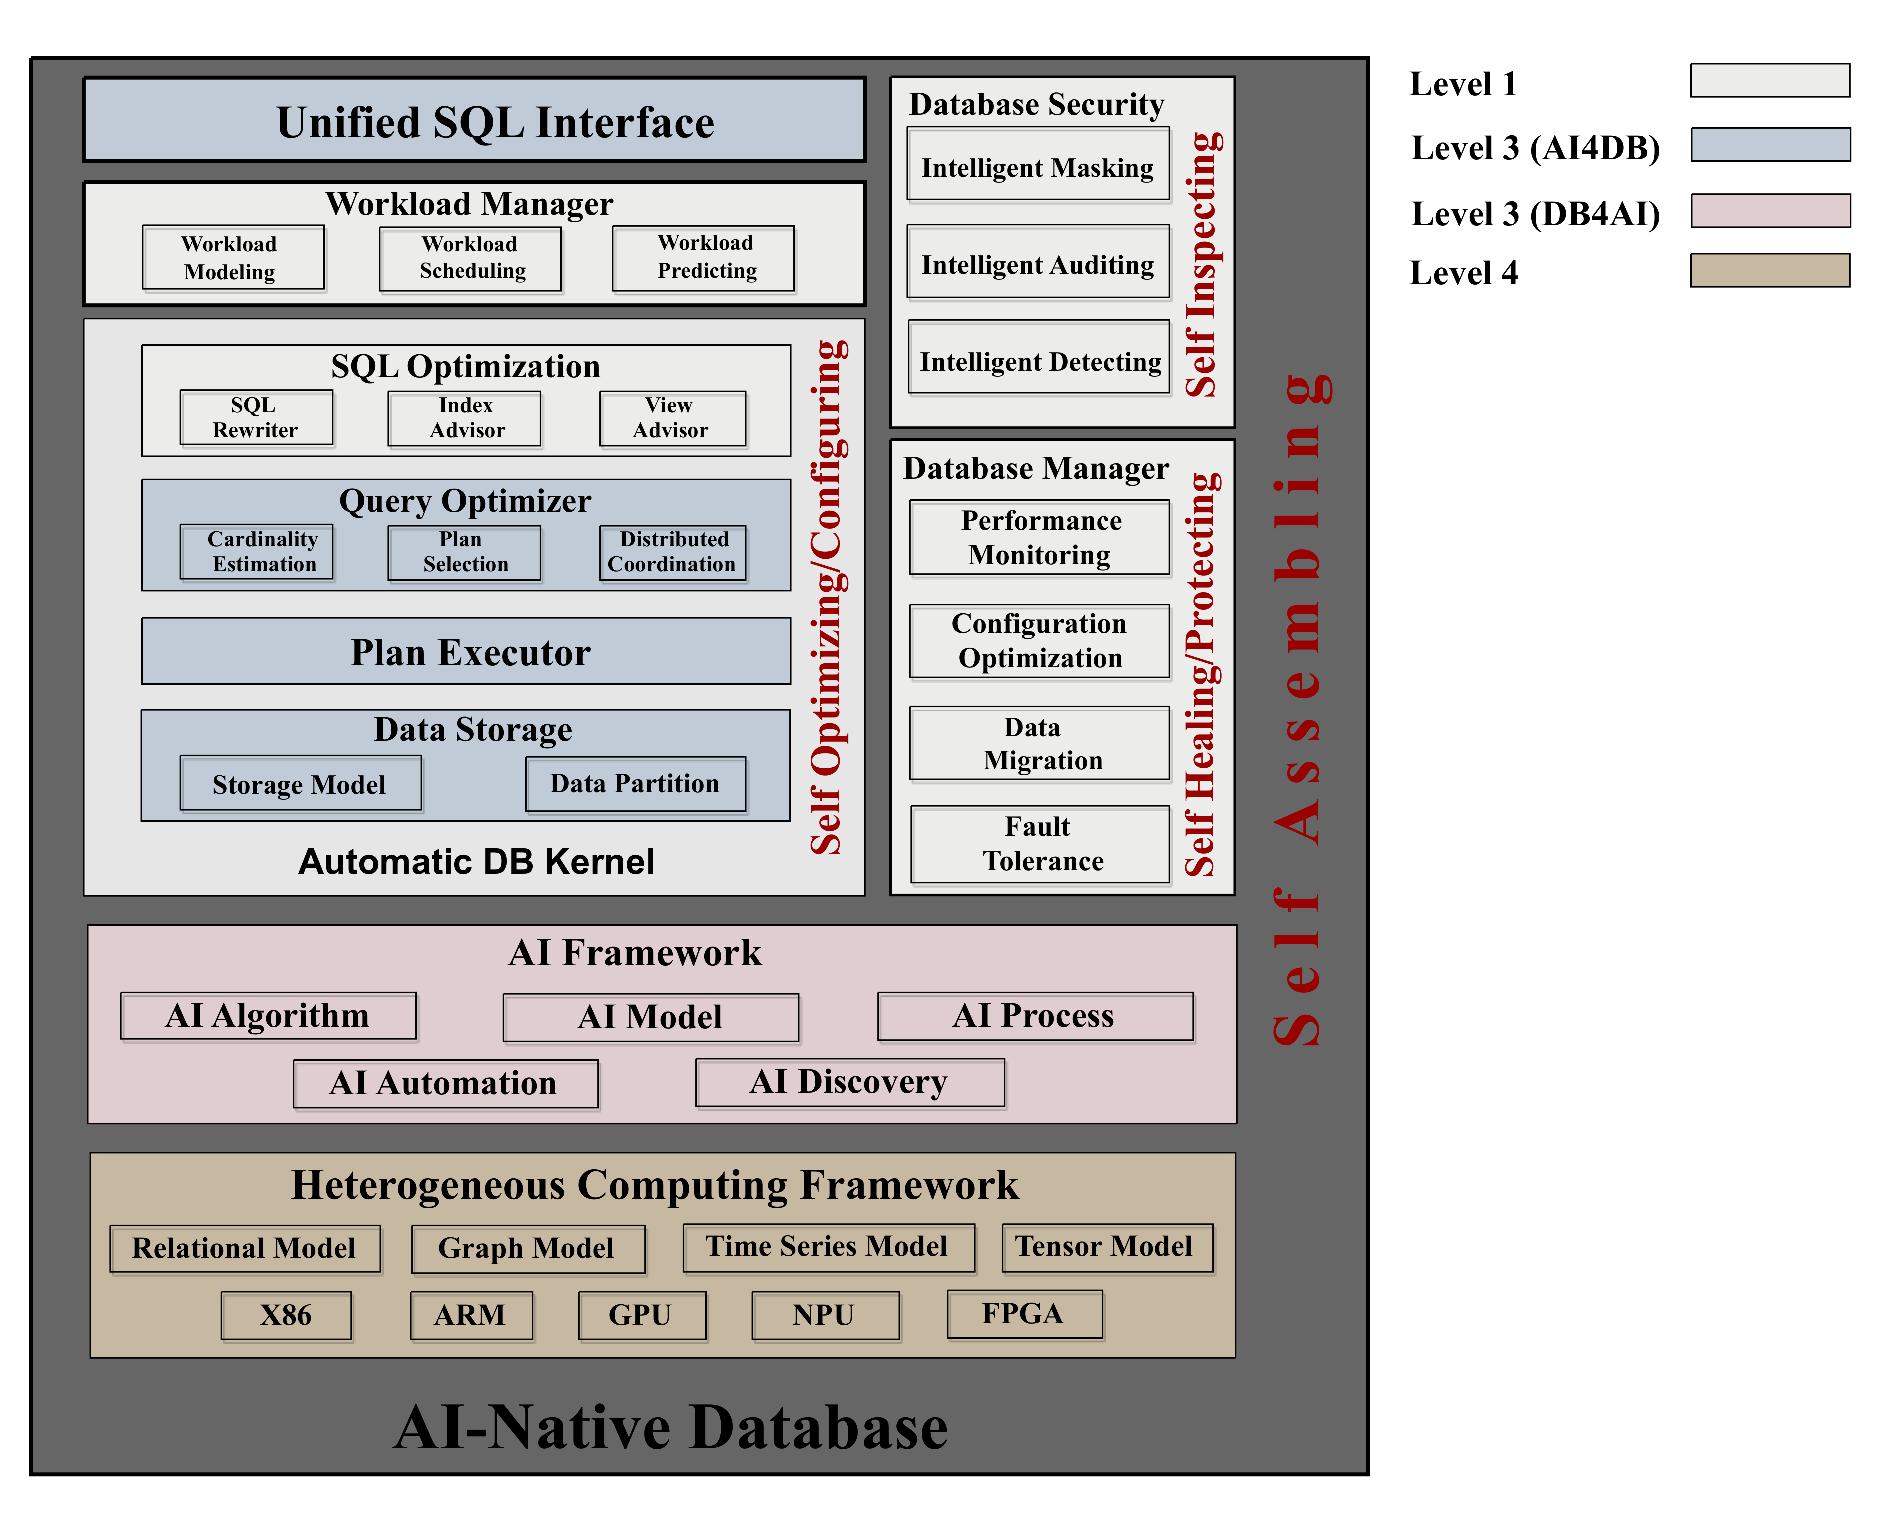
\includegraphics[width=1.0\textwidth, height=0.92\textwidth]{figs/ANDB-arch.eps}
\vspace{-1em}
\caption{The architecture of AI-Native databases}
\label{fig:ANDB}
\vspace{-1em}
\end{figure*}

 
To alleviate the issues talked above, in this section we propose a design of AI-native database, which better provides DB and AI services in five levels. 


\subsection{Level 1: AI-Advised Database}
\label{subsec: advised}
As shown in Table~\ref{tbl:ANDB}, in the first level, our database is AI-Advised, which provides auxiliary optimization of the database through suggestions~\cite{DBLP:conf/sigmod/AkenPGZ17, DBLP:journals/corr/abs-1802-00884, DBLP:conf/vldb/qtune19}.
It has an AI engine packing AI tools, which are loosely coupled with database in the form of plug-in. Limited by available resources, the AI engine mainly provides auxiliary tools from four aspects. 

$\circ$ \textbf{Workload Management}. It has two functions: to schedule user workloads and summary workload characters for the other modules. 
For \texttt{workload modeling}, traditional cost models are mostly based on empirical formulas, which have poor adaptability to different physical environments. Therefore, the machine learning model can be used to analyze and evaluate the current workload situation and future overhead, and dynamically adapt to the external environment based on gradient changes.
For \texttt{workload scheduling}, in traditional databases, resource scheduling depends heavily on parameters related to resource control, such as workspace size, maximum concurrent IO number, and etc. But these parameters are static and need to be manually configured. So we can use reinforcement learning to learn relations between database state (physical/logical), workload and database resources, and provide a reasonable and robust scheduling mechanism.
For \texttt{workload predicting}, workload usually dose not change in a fixed pattern. Traditional workload predicting methods are usually grasped by database experts according to statistical data, which can not guarantee high accuracy. So we proposed to use machine learning method for workload forecasting~\cite{DBLP:conf/sigmod/MaAHMPG18}, which can have better adaptability to different workloads. 
%In order to avoid using CPU, IO and other system resources as workload metrics in different hardware environments, we use logical metrics to characterize workload, which further ensures the stability of prediction.

$\circ$ \textbf{SQL Optimization}. It is to optimize database in SQL level. 
For \texttt{SQL rewriter}, SQL rewriter helps optimizer to choose efficient query plans by changing the way SQL is written. This level is often completed manually, which is impractical for heavy workload. So we provide a rewriting tool to learn the principles of SQL writing (e.g., avoiding full table scanning, selecting indexed columns as joins, and using table variables) and optimize the SQL structure. 
For \texttt{index advisor}, index is very important to improve the efficiency of retrieval tasks on complex data sets~\cite{DBLP:journals/kais/GaniSSH16}. However, the commonly used indexes are universal data structures. They do not analyze and utilize the distribution of data. So through machine learning, we can learn a model that reflects data patterns, and can automatically synthesize a special index structure at a lower cost.
For \texttt{view advisor}, given a set of queries, extracting high-frequency sub-queries and establishing materialized views to improve the performance of the database is very helpful. 
The traditional method caches at the whole query level, and the hit rate is low.
We construct the ML algorithm of sub-query selection according to the actual constraints so as to improve the query efficiency of batch SQL tasks.

$\circ$ \textbf{DB Manager}. It provides services (e.g., performance monitoring, tuning, fault tolerance) to ensure the stable operation of the database. In distributed scenario, high load pressure will lead to a sharp increase in failure rate, which brings great challenges to database maintenance. 
For \texttt{performance monitoring}, it automatically monitors the status of the database system (e.g., the number of batch requests per second, the number of user connections, network transceiver efficiency). Then it analyzes those indicators using machine learning algorithms. 
%Generally speaking, it includes four kinds of methods: real-time monitoring, timing monitoring, analysis report, tracking and data collection. Performance monitoring is not only statistical indicators, but also needs to understand the operation of the system based on these indicators. 
For \texttt{tuning}, database configuration involves hundreds of tunable system parameters, which control the database components in many aspects. Traditional tuning methods~\cite{DBLP:journals/pvldb/DuanTB09, DBLP:conf/cloud/ZhuLGBMLSY17} either relies on human beings (DBA-based), or cannot utilize history information (search-based). So we use a deep-reinforcement-learning-based tool~\cite{DBLP:conf/vldb/qtune19} to learn relations between database state, query and parameters, which can adapt to environment changes dynamically.
For \texttt{fault tolerance}, it includes a variety of strategies for resolving failures of hardware, transactions and system. In case of data error, the system needs to cancel the corresponding transactions in time. So we use a ML-based tool to monitor the changes caused by typical failures and realize pre-alerts. 

$\circ$ \textbf{DB Security}. It is to combine information security, cryptography technology with AI tech to  ensure the security of database. 
For \texttt{intelligent masking}, it is to hide privacy data such as ID number.  Intelligent masking technology only uses the high-dimensional, non-linear data inside the neural network to help improve the effect of data hiding. For example, in the research project conducted by Stanford University and Google, satellite images have been converted into high-frequency signals that are not easily detected. 
For \texttt{intelligent auditing}, it optimizes the auditing work from two aspects: data preprocessing and dynamic analysis. Traditional audit work often requires auditors to obtain a large number of business data. This part of the data understanding work is a waste of human resources. Intelligent auditing not only saves manpower cost, but also helps auditors to make better decisions by providing useful information from massive data.  
For \texttt{intelligent detecting}, it can automatically detect system vulnerabilities. Known intelligent detecting technology is mainly to retrieve through security scanning, while unknown security vulnerabilities need to do a lot of retrieval and testing work.  Using machine learning algorithm to discover security vulnerabilities~\cite{DBLP:journals/corr/abs-1902-10680}, it can not only detect most known vulnerabilities in national vulnerability database, but also predict and evaluate potential vulnerabilities.

\subsection{Level 2: AI-Assisted Database}
\label{subsec: assisted}
In the second level, our database is AI-Assisted, which is embedded into the database kernel for runtime optimization. AI components (e.g., tuning model, workload scheduling, view advisor)  can be merged into the corresponding database components~\cite{DBLP:journals/corr/abs-1903-01363}. This way, AI processes are integrated into the working procedure of the database. For example, if embedding the tuning model into the query optimizer, every time we generate the query plan, we can first conduct query tuning (adjust user-level parameters to better adapt to the incoming query characters), and then normally generate and execute query plan. The advantage of AI-Assisted database is that 1) it can provide more fine-grained optimization; 2) by embedding AI engine into the kernel, it can reduce much overhead such as communication cost.

However, neither Level 1 or 2 is a real AI-native database. Because the main components and organizing mode in those databases are still based on traditional methods. There are huge gap between AI technologies and databases. Starting from the third level, we introduce how to integrate intelligence integration, heterogeneity into database design to achieve the AI-native database.

\subsection{Level 3: AI-Enhanced Database}
\label{subsec: enhanced}
In the third level, our database is AI-Enhanced, which embeds intelligence and integration into database design. 
Firstly, we propose an intelligent database kernel, which implants AI into the design of database kernel. Secondly, we propose a  unified engine for both AI and DB, with which clients can use AI as easily as they use a DB.

\subsubsection{Intelligent Database Kernel}
\label{subsubsec: intelligent}
We present the design of an intelligent database kernel that enables self-configuring, self-healing, self-optimizing, self-protecting, self-inspecting and finally achieves self-organizing.

$\circ$ \textbf{Self-configuring}. Database can automatically adjust their own configuration to adapt to environment changes, including tuning parameters, upgrading software,adjusting partitioning/replication scheme, reorganizing tablespace and etc. Each function is embedded into particular DB modules to work as part of the processing.  For example, to realize tuning in query level, we embed tuner into optimizer. Each time a parse tree is input into our optimizer, it first configures parameters based on the query features and then actually generates the query plan. This way, it not only helps to generate better query plan, but prepares suitable environment for executing the query plan. 

$\circ$ \textbf{Self-healing}. Database can automatically detect, diagnose, alert and recover from DB problems (e.g., poor performance, hardware/software failovers). It adopts advantages of tools in AI-Advised DB to fully save humans from the failure-recovery loop. Firstly, it takes protective actions ahead of time (e.g., backup, data sharding, reosurce scheduling). Secondly, it can recover services even if emergency occurs (e.g., live migration).


%For example, rather than cleaning dirty pages in memory every fixed time, we replace the timing part  with the results of workload forcasting, which can predict how the workload varies. And it conducts cleaning when DB is free.live migration, checkpoint,  logging each write operations, we can focus on recording 

$\circ$ \textbf{Self-optimizing}. Database can automatically collect statistics of queries and optimize database performance in multiple granularities. Firstly, it collect statistics used in optimizer to learn current workload, which can benefit from cardinality estimation and workload scheduling. Secondly, it automatically design index, materialized query table (MQT) and data partition, which can directly optimize performance of single query. Thirdly, it automatically controls the flow of queries with query patroller to achieve overall optimization.

$\circ$ \textbf{Self-protecting}. Database can automatically monitor processing procedure of each query and prevent potential damage in time. For example, it can throttle service requests which compete resources to cut down deadlock and average waiting time; and it can kill / lower the priority of run-away queries (execution time is far longer than that estimated by the optimizer) to prevent from using up system resources.

$\circ$ \textbf{Self-inspecting}. Database can automatically monitor database state and conclude operating rules by itself. It can check database state (e.g., data consistency, DB health) all the time. And by concluding all the failover conditions and solutions, it can translate the experience in the form of publication of instrumentation data in favor of human understanding.


$\circ$ \textbf{Self-organizing}. For current databases, each level of service (e.g., parser, optimizer and executor) has multiple standardized components to choose from. How to choose the appropriate processing path for one or a batch of queries becomes meaningful. 

So we propose a self-organizing module. For different queries, we can dynamically select the appropriate components in each layer of service and assemble the appropriate execution path.
The execution path can be seen as a natural language sequence (NLS), such as $\langle$ $SQL_i$, parser$\_$pg, optimizer$\_$RBO, storage row, accelerator $\rangle$, in which each position has only discrete token options. So the problem is how to generate NLS in query level. One method is to use RL algorithm. It takes the whole path sequence as an episode and a single action as an epoch. Under each epoch, the agent chooses the next component (action), which executes the query, leading to a state transition (e.g., the query status changes into syntax tree). In this problem, action is discrete, so DDQN algorithm~\cite{DBLP:conf/aaai/HasseltGS16} can be used. Compared with other RL algorithms with discrete output, DDQN eliminates the problem of overestimation (deviate greatly from the optimal solution) by choosing decoupling actions and calculating the target Q value.

However, RL-based routing algorithm has two problems. 
Firstly, Q network will not score until the last node is generated. It is insensitive to the choice of intermediate nodes. However, for the entire path, it is necessary to give action a comprehensive score on current and future impacts. 
Secondly, when training with epoch as a unit, each node of a path is scattered in a training sample, instead of being used as a whole to calculate the gradient. 

Generating antagonistic network (GAN)~\cite{DBLP:journals/corr/abs-1902-05687} can better solve those problems of end-to-end path selection. We use G network to generate path vectors based on workload, database state and component characteristics, and we use D network as the performance model. 
But the traditional GAN network model is not fully applicable to our problem. Because it is mainly used to generate data with continuous range of values, and it is difficult to generate path vectors with discrete tokens. That is because G-networks need to be fine-tuned based on gradient descent and regress towards the expectation. But when the data is discrete tokens, fine-tuning is often meaningless.
So we choose to combine RL algorithm with GAN~\cite{DBLP:conf/aaai/YuZWY17}. Firstly, G network is used as agent in RL algorithm: action is the next service node; state includes not only query status, database status, but also generated node information. Each iteration generates a complete path. Secondly, unlike pure RL algorithm, each action is scored by D network to guide the generation of the whole path sequence.

\subsubsection{Unified Engine for AI and DB}
\label{subsubsec: engine}
After achieving the intelligent database kernel, we gain real integration by providing unified engine for DB and AI. AI and DB are closely connected. For DB, as talked above, AI can make DB  smarter. For AI, DB stores large scale of data for training the ML models. 
So it becomes easy when we can call ML model with SQL statements. Firstly, SQL is easy to use, with which technicians with basic SQL knowledge can complete most of traininig and predicting tasks. Secondly, it saves people from frequently switching between different languages of systems, when we need to write SQL to fetch data and run python scripts to run ML algorithms.

For this work, there have been some products such as BigQuery ML~\cite{DBLP:conf/ideas/FernandesB15}, SQL for DL and SQLFlow. Considering the Pros and Cons of these works, we propose an extended DB engine to achieve the following aims:

$\circ$ \textbf{AI Support}. Firstly, SQL Parser should extend SQL syntax to utilize AI methods, including model creating, training and predicting. Besides, it should minimize the use of other scripting languages (e.g., Python and R). Secondly, we extend the relational algebra theory to support both relational and tensor data models. This way, DB can support tensor processing, which is largely used in the training of AI models.


$\circ$ \textbf{General Purpose}. SQL parser should contain an abstract layer which maintains a loose couple with lower components. This way, it can be easily used on different SQL engines (e.g., PostgreSQL, Flink and Hive) or machine learning toolkits (e.g., TensorFlow, Keras and scikit-learn). 

$\circ$ \textbf{Custom Style}. Besides general operators such as SELECT and WITH, we also allow user to define how to train, evaluate and predict the ML models with user-defined functions. And they also can cache the trained model with materialized views.

The general workflow is as follows. Firstly, SQL Parser parses a SQL statement and produces a general-purpose query plan. Based on the operators in the plan, it decides whether it is for manipulating data or calling ML models. If for manipulating data, the query plan is sent to the DB executor and be executed. Otherwise, it is sent to the AI executor and be executed.

This way, database can also provide AI services in an end-to-end way. As table~\ref{tbl:AI} shows, Database supports AI services in five levels.
%Presently, DB mainly serves for structured data analysis such as financial transactions. By embedding AI algorithms into DB engine, DB can directly support many AI applications (e.g., image comparison, graph computing) in an end-to-end way. As Figure~\ref{fig:DB4AI} shows,  

$\bullet$ \textbf{DB-based AI Algorithm}. Database provides ML tool-kits and libraries (e.g., TensorFlow, Scikit-learn). Clients can write AI algorithms in UDFs or stored procedures. And they can call them repeatedly from database. 

$\bullet$ \textbf{DB-based AI Model}. Database provides classic AI models (e.g., random forest, RNN, DDQN). Clients can directly call AI models from database and only focus on the training part. 

$\bullet$ \textbf{DB-based AI Process}. Database further provides AI processes, which not only include the mature AI models but the training methods (e.g., SGD, Adam, reinforcement learning). Clients can directly call AI processes from database, only with data as input. Database automatically fine-tunes AI model using corresponding training method, and utilizes the model to produce results. 

$\bullet$ \textbf{DB-based Automation}. Database can automatically parse the requirements in AI and call proper process to solve it. Clients only need to declare their requirement. For example, if we hope to search some images, we just declare the conditions and data sources with SQL. And database automatically chooses the CNN model to conduct the work, which is also a part of the query plan.

$\bullet$ \textbf{DB-based Discovery}. Database offers an insight into the data schema and application queries, and optimizes itself with AI techniques. For example, if a new workload comes, database can call a DRL-based tuner to adjust the system parameters based on the query features, including cost estimation, resource allocation, concurrency  control and etc. 

\begin{table}[h]
\vspace{-1em}
\centering
\caption{Five levels of machine learning consumability in DBMS}
\label{tbl:AI}
{%\footnotesize
  \hspace*{-0em} \begin{tabular}{|c|c|l|c|c|}\hline
  
\multirow{2}{*}{\textbf{Level}} & \multirow{2}{*}{\textbf{Consumability}} & \multirow{2}{*}{\textbf{\ \ \ \ \ \ \ \ \ \ \ \ \ \ \ \ \ \ \ \ \ \ \ \ Description}} & \multirow{2}{*}{\textbf{Target Users}} & $\textbf{ML Skill}$ \\
 &  &  & & $\textbf{Level}$ \\\hline

\multirow{2}{*}{\textbf{1}} & \multirow{2}{*}{Algorithm} & \multirow{2}{*}{Algorithms as UDFs and stored procedures} & Data scientists,  & \multirow{2}{*}{High} \\
 &  & & experienced developers & \\\hline


\multirow{2}{*}{\textbf{2}} & \multirow{2}{*}{Model} & Models as first-class object with DDL, & App. developers  & \multirow{2}{*}{Medium} \\
 &  &  DCL, DML capability  & and DBAs & \\\hline

\multirow{2}{*}{\textbf{3}} & \multirow{2}{*}{Process} &  Processes as first-class object with DDL, & App. developers & \multirow{2}{*}{Low} \\
 &  & with DCL, DML capability  & and DBAs & \\\hline

\multirow{2}{*}{\textbf{4}} & \multirow{2}{*}{Automation} &  Problem specifications as first-calss object & Business specialists, DBAs & \multirow{2}{*}{Low} \\
 &  & with DDL, DCL, DML capability  & app. developers & \\\hline


\multirow{2}{*}{\textbf{5}} & \multirow{2}{*}{Discovery} &  Discover ML opportunities based on & Business specialists, DBAs & \multirow{2}{*}{Very Low} \\
 &  & data schema and application queries  & app. developers & \\\hline

  
  \end{tabular}
}
\vspace{-1em}
\end{table}

\subsection{Level 4: AI-Assembled Database}
\label{subsec: assemble}
In the fourth level, our database is AI-Assembled, which embeds heterogeneity into database design. That is ,we assemble AI with database by supporting multiple leading computing powers. We know traditional database is only based on CPU. However, DB and AI technology usually require different computing power and hardware. For DB, traditional optimizer processes queries with CPU. While AI technology requires new chips to support parallely processing (e.g., GPU and NPU) and self-scheduling. And now many applications need to use both DB and AI technology, especially in large data analysis scenarios.

AI-assembled database mainly has two contributions. Firstly, it can support ARM architecture. 
1) It effectively utilizes ARM array with multi-core mode, inter-node parallelism, intra-node parallelism, instruction-level parallelism, compiler parallelism and other super-parallel technologies. 
2) For the problem of competition brought by multi-core, it provides cross-chip access optimization and resource scheduling optimization. 
Secondly, it can utilize different computing powers to better serve the AI components. It is able to switch computing powers based on the processing types. For example, for the tuning module in optimizer, when training the tuning model, we fetch training data into memory with ARM and conduct backward propagation (training the neural network) with NPU. And database should flexibly schedule computing powers, e.g., when NPUs are overburdened but most ARM resources are idle, ARM array can share some burden.

The ultimate objective of this database is to fully unleash the power of diversified computing, which includes x86, ARM, GPU, NPU, and accelerators. We aim to continuously push our AI strategy forward and foster a complete computing ecosystem. 


\subsection{Level 5: AI Designed Database}
\label{subsec: designed}
In the last level, AI technology is integrated into the whole database life cycle (DBLC) of our database so as to achieve the ultimate goal of scenario-aware and AI-as-a-Service. The whole life cycle includes five phases: 1) Database initialization; 2) Database design; 3) Database implementation; 4) Database evaluation; 5) Database operation and maintenance.


\begin{table}[h]
\vspace{-1em}
\centering
\caption{Five levels of AI-native database}
\vspace{0.5em}

\label{tbl:ANDB}
{%\footnotesize
  \hspace*{-0em} \begin{tabular}{|c|c|l|l|}\hline
  
\multirow{1}{*}{\textbf{Level}} & \multirow{1}{*}{\textbf{Feature}} & \multirow{1}{*}{\textbf{\ \ \ \ \ \ \ \ \ \ \ \ Description}} & \multirow{1}{*}{\textbf{\ \ \ \ \ \ \ \ \ \ \ \ \ \ \ \ \ \ \ \ \ \ \ \ \ \ \ \ \ \ \ \ \ \ \ \ Example}} \\\hline

\multirow{4}{*}{\textbf{1}} & \multirow{4}{*}{AI-advised} & \multirow{4}{*}{ plug-in AI engine} &$\circ$ Workload Manager (e.g., \small{workload scheduling/predicting})  \\
 &  & & $\circ$  SQL Optimization \small{(e.g., SQL rewriter, index/view advisor)} \\
 &  & &$\circ$  DB Maintenance \small{(e.g., knob tuner, fault tolerance)}\\
 &  & &$\circ$  Security \small{(e.g., intelligent masking/auditing/detecting)}\\\hline

\multirow{4}{*}{\textbf{2}} & \multirow{4}{*}{AI-assisted} & \multirow{4}{*}{Built-in AI engine} &$\circ$ Embed workload scheduling as job-queue mechanism \\
 &  & & $\circ$  Embed index advisor as an optional database indexing\\
 &  & &$\circ$ Embed knob tuner as a self-adaptive module \\
 &  & &$\circ$  Replace database auditing with intelligent auditing \\\hline

\multirow{7}{*}{\textbf{3}} & \multirow{7}{*}{AI-enhanced} & \multirow{7}{*}{Hybrid DB\&AI engine} &$\circ$ Intelligent Database Kernel \\
 &  & &\ \ \  $\bullet$ Self-configuring (e.g., self tune/upgrade/data partition)\\
 &  & &\ \ \  $\bullet$ Self-healing (e.g., self failover/alert/recovery)\\
 &  & &\ \ \  $\bullet$ Self-optimizing (e.g., collect stats, design index/MQT)\\
 &  & &\ \ \  $\bullet$ Self-protecting (e.g., throttle run-away queries )\\
 &  & &\ \ \  $\bullet$ Self-inspecting (e.g., consistency/health check)\\
 &  & &\ \ \  $\bullet$ Self-organizing (e.g., form executing path in query level)\\
 &  & &$\circ$ Unified Engine for AI+DB \\\hline

\multirow{2}{*}{\textbf{4}} & \multirow{2}{*}{AI-assembled} & \multirow{2}{*}{Heterogeneous computing} &$\circ$ Support new hardware (e.g., ARM, GPU, NPU) \\
 &  &   &$\circ$  Extend relational algebra to support tensor model \\\hline

\multirow{5}{*}{\textbf{5}} & \multirow{5}{*}{AI-designed} & \multirow{5}{*}{The life cycle is AI-based} &$\circ$ Database initialization \\
 &  & & $\circ$  Database design\\
 &  & &$\circ$ Database implementation and loading\\
 &  & &$\circ$  Database testing and evaluation \\
 &  & &$\circ$  Database operation and maintenance \\\hline
  
  \end{tabular}
}
\vspace{-1em}
\end{table}




%!TEX root = ../main.tex

\section{Challenges and Opportunities}
\label{sec: challenge}

It brings new research challenges and opportunities to design an AI-native database, which aims to support data management, data analysis, machine learning together in the same system.

\subsection{From one-size-doesn't-fit-all to one-stack-fits-all}

Michael Stonebraker argues that one size does not fit all, due to various applications (e.g., OLTP, OLAP, stream, graph) and diversified hardware (e.g., CPU, ARM, GPU, FPGA, NVM). Note that the database components and their variants are limited, but the number of possible combinations for these components to assemble a database is huge. So the database architects design the database architectures by combining different variants of techniques based on their empirical rules and experience. Thus these human-designed databases may not be optimal because they may fall into a local optimum. It calls for automatically designing a database using AI techniques, which can adapt to different scenarios. 


We argue that one stack fits all. The basic idea is to first implement the database components, e.g., indexes, optimizers, storage, where each component has multiple variants/options, then use AI techniques to assemble these components to form some database candidates, and finally select a database that best suits a given scenario. In this way, we can automatically verify different possible databases (i.e., different combinations of components), explore many more possible database designs than human-based deign, and could design more powerful databases. This is similar to AlphaGO, where the learning-based method beats humans, because the machines can explore more unknown spaces. 


There are several challenges in one-stack-fits-all. First, each component should provide standard interfaces such that different components can be integrated together. Second, each component should have different variants or implementations, e.g., different indexes, different optimizers. Third, it calls for a learning-based component to assemble different components. Fourth, the assembled database can be evaluated and verified before the database is deployed in real applications.  Fifth, each component should be run on different hardware, e.g., learned optimizers should be run on AI chips and traditional cost-based optimizers should be run on general-purpose chips. It calls for effective methods to schedule the tasks. 


\subsection{Next Generation Analytic Processing: OLAP 2.0}

Traditional OLAP focuses on relational data analytics. However, in the big data era, many new data types have emerged, e.g., graph data, time-series data, spatial data, it calls for new data analytics techniques to analyze these multi-model data. Moreover, besides traditional aggregation queries, many applications require to use machine learning algorithms to enhance data analytics, e.g., image analysis. Thus it is rather  challenging to integrate AI and DB techniques to provide new data analytics functionality. We think that hybrid DB and AI online analytic processing on multi-model data should be the next generation OLAP, i.e., {\it OLAP 2.0}. 

There are several challenges in supporting OLAP 2.0. First, different data types use different models, e.g., relational model, graph model, KV model, tensor model, and it calls for a new model to support multi-model data analytics. Second, OLAP 2.0 queries may involve both database operations and AI operations, and it needs to design new optimization model to optimize these heterogeneous operations across different hardware. 



\subsection{Next Generation Transaction Processing: OLTP 2.0}

Traditional OLTP mainly uses general-purpose hardware, e.g., CPU, RAM and Disk, but cannot make full use of new hardware, e.g., AI chips, RDMA, and NVM. Actually, we can utilize new hardware to improve transaction processing. First, based on the characteristics of NVM, including non-volatile, read-write asymmetry speed, and wear-leveling, we need to reconsider the database architecture. For example, we can utilize NVM to replace RAM and replace page-level storage with record-level storage on NVM. Second, we can utilize RDMA to improve the data transmission in databases. Moreover, we can use the programmable feature of intelligent Ethernet card to enable filtering on RDMA and avoid unnecessary processing in RAM and CPU. Third, there are some AI chips which are specially designed hardware, and it is also promising to design database-oriented chips that are specially defined hardware for databases. 


There are several challenges in supporting OLTP 2.0. First, it is challenging to fully utilize new hardware to design a new generation database. Second, it is hard to evaluate and verify whether the new hardware can benefit the database architecture. Third, it calls for an effective tool to automatically evaluate a feature or a component (even a database). 




% Fifth, each component should be run on different hardware, e.g., learned optimizers should be run on AI chips and traditional optimizers should be run 




\subsection{AI4DB}

There are several challenges that embed AI capabilities in databases. 

\hi{Training Samples.} Most AI models require large-scale, high-quality, diversified training data to achieve good performance. However, it is rather hard to get training data in databases, because the data either is security critical or relies on DBAs. For example, in database knob tuning, the training samples should be gotten based on DBAs' experiences. Thus it is hard to get a large number of training samples. Moreover, the training data should cover different scenarios, different hardware environments, and different workloads.  

% Moreover, the training data must be high quality, number and diversity of samples.

\hi{Model Selection.} There are lots of machine learning algorithms and it is hard to automatically select an appropriate algorithm for different scenarios. Moreover, the model selection is affected by many factors, e.g., quality, training time, adaptability, generalization. For example, deep learning may be a better choice for cost estimation while reinforcement learning may be a better choice for join order selection. The training time may also be important, because some applications are performance critical and cannot tolerate long training time. 

%, which usually cannot be satisfied in database. Second, any AI model needs relatively long training time, which is usually intolerable in database.

\hi{Model Convergence.} It is very important that whether the model can be converged. If the model cannot be converged, we need to provide alternative ways to avoid making bad decisions. For example, in knob tuning, if the model is not converged, we cannot utilize the model for knob suggestion.   
 
\hi{Adaptability.} The model should be adapted to different scenarios. For example, if the hardware environments are changed, the model can adapt to the new hardware. 
  
\hi{Generalization.} The model should adapt to different database settings. For example, if the workloads are changed, the model should support the new workloads. If the data are updated, the model should be generalized to support new data. 
 

\subsection{DB4AI}

\hi{Accelerate AI algorithms using indexing techniques.} Most of studies focus on the effectiveness of AI algorithms but do not pay much attention to the efficiency, which is also very important. It calls for utilizing database techniques to improve the performance of AI algorithms. For example, self-driving vehicles require a large number of examples for training, which is rather time consuming. Actually, it only requires some {\it important examples}, e.g., the training cases in the night or rainy day, but not many redundant examples. Thus we can index the samples and features for effective training. 


\hi{Discover AI Models.} Ordinary users may only know their requirements, e.g., using a classification algorithm to address a problem, but do not know which AI algorithms should be used. Thus it is important to automatically discover AI algorithms. Moreover, it is also challenging to reuse the well-trained AI models by different users. 



\subsection{Edge Computing Database.} Most databases are designed to be deployed on servers. With the development of 5G and IOT devices, it calls for a tiny database embedded in small devices. There are several challenges in designing such a tiny database. The first is database  security to protect the data. The second is real-time data processing. The small device has low computing power, and it is rather challenging to provide high performance on such small devices. The third is data migration among different devices. Some devices have small storage and it is challenging to migrate the data across different devices. 



%\hi{Security}

%\hi{Database function As a Service}



%, and deploy the  automatically designed database for different .  

%Note that different databases usually adopt the common techniques, e.g., index and cost-based optimizer, but 

%The database architects 
%As Figure~\ref{fig:ANDB} shows, AI-native database can support AI and DB services naturally and efficiently. It brings new opportunities to the development of database. However, due to the demands of AI algorithms (e.g., training data), as well as problems in DB technology itself, there are still several challenges in the process of deploying such a design.

%\subsection{Challenges in AI}
%\label{sec: ch-AI}
%Challenges in AI is mainly around two aspects. First, any AI model needs large-scale and high-quality training data to achieve good performance, which usually cannot be satisfied in database. Second, any AI model needs relatively long training time, which is usually intolerable in database.

%\subsubsection{Lack of training data}
%\label{subsec: data}
%AI algorithms rely on training data heavily, including the quality, number and diversity of samples.

%$\bullet$ \textbf{Sample Quality}. Sample quality has the most direct impact on the quality of model training. In order to train the prediction model correctly, the sample data must be correct and de-duplicated. But it is difficult to guarantee the data quality in the database system. Firstly, although the database system has abundant statistical information, many of these information are not real-time updates, such as the statistical information of relational tables. Secondly, these data will be affected by many factors, such as cardinality estimation, not only the data distribution information of relational tables, but also the execution cost of various physical operations of the database.

%$\bullet$ \textbf{Sample Number}. High quality samples alone are not enough to train robust AI models. Taking neural network as an example, if the training samples are very small and the number of updates of connection weights is small, the space that the model can explore is very limited. And the adaptability of the model can be weak. While in DB, many problems can hardly provide enough training samples. For example, for workload forecasting, user data in real scenarios are often hard to get, under strict protection.

%$\bullet$ \textbf{Sample Diversity}. Although the mature machine learning model can adapt to new problems, providing typical samples in training stage can accelerate the convergence speed of the model and improve the accuracy and adaptability of the model. However, in database-related problems, due to the limited training time allowed, it is often difficult to obtain sufficient and diverse data in the initial training stage. For example, in the tuning problem, the training stage often only provides several typical benchmark workloads.

%\subsubsection{Unaffordable Training Time}
%\label{subsubsec: time}
%Data alone is not enough for machine learning. The learning model needs enough training time to transform input knowledge into output knowledge. Therefore, in fact, simple classifiers can be widely used, because training complex classifiers takes a long time. Similarly, it is difficult for database systems to converge when they are faced with various user needs. Therefore, there are two requirements for the selection of machine learning algorithm in database system. First, the model adapts to the scenario. For example, in tuning problem, many parameters have continuous ranges of values, and algorithms such as Q-learning need to keep large-scale tables, which wastes time and resources. Secondly, it combines gradient descent and transfer learning to improve training efficiency. Up to now, many algorithms have been proposed to optimize training efficiency. For example, in reinforcement learning, Actor-Critic algorithm can enhance the convergence speed with the Critic evaluating the behavior of the Actor.

%\subsection{Challenges in DB}
%\label{sec: DB}
%Here we mainly consider the challenges that DB can bring about to AI. There are three problems.

%\subsubsection{Various Hardware}
%\label{subsec: hardware}
%The challenges of the hardware environment include two aspects. 

%$\bullet$ Hardware on which database processes transactions. New computing and storage media are emerging, with ROM like  SSD, disk array, NVM and CPU architectures like SMP, AMP. People often configure different for thier databases, considering many factors (e.g., budgets, applications). And in cloud environment, much more hardware instances exist. Different hardware environments can have a great impact on AI technology. For example, in knob tuning, many parameters are strongly related to hardware, such as the cost of reading/writing tuple, the overhead of database operators and so on. The model will take a long time to correct the historical cognition without taking the hardware changes into consideration. 
%For example, in cardinality estimation technology, if the system supports multiple threads (workers) to execute a query plan in parallel, the relationship between operator overhead at different levels is no longer simple summation. Machine learning model needs more time to adapt to the change of implicit rules. 

%$\bullet$ Hardware on which AI model is trained. In order to reduce the time used to train large-scale machine learning models, Intel, Google, Microsoft and other manufacturers have released a variety of hardware specifically to help train AI models (e.g., GPU, TPU, FPGA). Altough those hardwares improve the efficiency of matrix computing, they require the corresponding adjustment of machine learning algorithm to adapt. For example, For example, if you want to migrate an AI model from CPU to GPU, you need to migrate tensors, variables and the model to the display memory in GPU.

%\subsubsection{Various Workload}
%\label{subsec: workload}
%Various workloads pose challenges in two aspects.

%$\bullet$ With different workloads, the database not only needs to provide appropriate operation and maintenance strategy, execution plan, processing flow, but also needs to provide appropriate architecture to store data. For example, in edge computing, we need to provide services nearby, and there are some problems such as data/service migration; in cloud database, it manages data uniformly and maintains diverse distributed clusters. Firstly, that requires AI model to filter out the important factors in the workload, and dynamically adapt to changes. 

%$\bullet$ Hybrid application services increase the complexity of database management.  Different workload types often correspond to different services, such as OLTP, OLAP and HTAP. And many applications require hybrid services. For example, banking system not only provides transactional business, but also needs analytical business such as data auditing and analysis. So database instances can no longer serve one type workload. This kind of composite business has higher requirements for database storage, processing and data management. This requires that the machine learning model trained from a single scenario can provide a good enough service for hybrid workload types.

%\subsubsection{Various User Requirements}
%\label{subsec: requirement}

%Different users often notice different database performance. For example, real-time services require low query latency, while batch services require high throughput. In order to guarantee the desired performance, databases often need to sacrifice the performance of other aspects. For example, in order to improve the utilization of the overall resources, the number of parallel connections can be increased, but the workspace allocated for each connection will be reduced, which will affect the execution efficiency of a single task. In cloud databases, there are a variety of user "preference". In order to use machine learning to optimize database technology, it is necessary that machine learning model can automatically and quickly adapt to the requirements of different users, and allocate resources reasonably based on priority. 
%And use various statistical, caching, data collation mechanisms (such as vacuum) to improve resource utilization and fault-tolerant disaster prevention capabilities, improve resource utilization and database stability, and further enhance user experience.




%!TEX root = ../main.tex

\section{Concluding Remarks}
\label{conclusion}

There exist many systems for monitoring and analyzing spatio-temporal data, such as a dashboard for visually tracking the outbreak of COVID-19~\cite{dong2020interactive} and a tweet stream sentiment analysis system for US election 2016~\cite{DBLP:conf/kdd/PaulLTYF17}. 
One lesson from the existing systems is  that they are usually designed on a case-by-case basis and built from scratch, which cannot fully leverage the recent techniques for data integration and automatic visualization.

On the one side, \sys-COVID-19 shares many common visualizations as the other popular websites for tracking COVID-19 cases.
On the other side, it differs from the others in 
(1) \sys-COVID-19 is based on a general end-to-end framework \sys, and leverages recent techniques for data preparation (\eg~{\sc VisClean}~\cite{visclean-icde}) and for visualization recommendation (\eg~{\sc DeepEye}~\cite{deepeyeicde});
%
(2) it supports linked visualization for the users to easily zoom in/out multiple visualizations by a single click; and
%
(3) it also obtains some private data that is not publicly available, so it can demonstrate some unique features.
%
%Hopefully we can survive the war of fighting COVID-19 with the minimum cost, and by the time of VLDB 2020, we will have much more to demonstrate.

%\add{Open Challenges: (1) Smart and Effective Data Preparation. (2) Data Sharing Platform. (3) Intelligent Data Analysis (4) Abstract general modules, the system supports reusability}
%%!TEX root = ../main.tex

\section{QUERY Clustering}
\label{sec:cluster}

For workloads including both transactional queries and analytical queries~\cite{DBLP:conf/icde/OhL05}, if the user aims to optimize the latency, we recommend  {\it query-level} tuning; if the user aims to improve the throughput, we recommend  {\it workload-level} tuning. For analytical only queries, we recommend cluster-level tuning to balance the throughput and latency. The key problem in the cluster-level tuning is (1) how to efficiently find the appropriate {\it configuration pattern} for each query and (2) how to cluster the queries based on the configuration pattern.  This section studies these two problems. % in this section.


\subsection{Configuration Pattern}
\label{sec:pattern}
The configuration pattern of a query should include all the knobs used in the DS-DDPG model. Thus a nature idea is to use DS-DDPG to generate a continuous knob configuration and take the knob configuration as the pattern. However it is rather expensive to get the continuous knob values, especially for a large number of queries. More importantly, when we cluster the queries, we do not need to use the accurate configuration pattern; instead approximate patterns are good enough to cluster the queries. 

\lgl{To this end, we discretize the continuous values into discretized values. For example, we can discretize each knob into \{-1,0,+1\}. Specifically, for each knob, if the tuned knob value is around the default value, we set it as 0; 1 if the estimated value is much larger than the default value; -1 if the estimated value is much smaller than the default value.}

\lgl{To avoid the curse of dimensionality when clustering queries, we only choose knobs most frequently tuned by DS-DDPG as the features, about 20 in PostgreSQL.} But the new knob space is still very large. For example, if \lgl{20} knobs are used and each has 3 possible values, then there are $3^{\lgl{20}}$ possible cases. The traditional machine learning methods or regression models are hard  to solve this problem, because they either assume the labels are independent such as Binary Relevance~\cite{DBLP:journals/pai/LuacesDBCB12} or cannot support so many labels such as Classifier chain~\cite{DBLP:journals/ml/ReadPHF11}. 



\vspace{.25em} 
\noindent {\bf  Learning Discrete Configuration Patterns Using Deep Learning.}  We choose the deep learning method to map queries to discrete configuration patterns. As Figure \ref{fig:DL} shows, the \texttt{Vector2Pattern} uses a neural network, which adopts a five-layer architecture. 

The input layer takes the feature vector as input and maps it to the target knob space, in order to make the input and output in the same scale. 

The second layer is designed to explore the configuration patterns. It is a dense layer with \lgl{ReLU} as the activation function %It expends the feature space by 2 times to explore more complex patterns. And  \lgl{ReLU}  
$(y = max(x, 0)$, where $x$ is an input feature and $y$ is the corresponding output features, using to learn two aspects of knowledge: 1) Interaction effects; 2) Non-linear effects. Interaction effects capture the correlations among the input features. For example, feature $v_i$ captures the value difference when other features' value changes. While Non-linear effects learns non-linear mapping relations between input vector and output vector. 

The third layer is a BatchNormal layer. It normalizes the input vector in favor of gaining discretized results. 

The fourth layer has the same function as the second and the value of each feature in this layer's output vector ranges from 0 to 1. But different from \texttt{Predictor} in Section~\ref{sec:tunner}, the last layer uses a {\it sigmoid}  activation function $S(z_{i})$ = $\frac{1}{1+e^{-z_{i}}}$, where $z_i$ is the $i_{th}$ feature of the input vector. It takes a real value as input and outputs a value in 0 to 1. This aims to do a non-linear data transformation and  at the same time keeps the features in the limited range.  

%\lgl{It is nonlinear, continuously differentiable and it changes monotonously.}  % To avoid sparing space causes too many $"$noise$"$ points, we also convert the knobs of numerical type into discrete values. 

For the DL model, we also append a step function to the network's end and use the output layer as a probability distribution function: for each feature $y$ in the output vector, the resulting bit is -1 if $y$ is below 0.5; 0 if $y$ equals to 0.5; and 1 otherwise. In this way, the DL model can automatically finish data transformation and discretization work. 

%\lgl{what is y?}\lgl{give more details of deep learning model!!!}


\begin{figure}[!t]\centering
\vspace{-.5em}
\includegraphics[width=.45\textwidth, height=.27\textwidth]{tuning_figs/DL_x.eps}
\vspace{-2em}
\caption{Architecture of the DL model}
\label{fig:DL}
\vspace{-2.5em}
\end{figure} 


\vspace{.25em} 
\noindent{\bf Workflow of \texttt{Vector2Pattern}.} 
The DL model works in 4 steps: 1) For each training sample $\langle q, p_r\rangle$, where $q$ is a query and $p_r$ is the real pattern that matches $q$,  compute the feature vector $v$ of query $q$; 2)  Propagate these features through its network; 3) Output an estimated  pattern $p_e$; 4) Based on the output pattern $p_e$ and the actual pattern $p_r$, update the weights in the network by minimizing $|p_e-p_r|$. 



\vspace{.25em} 
\noindent{\bf Training Step. } We need to generate a large volume of samples to train \texttt{Vector2Pattern} until the performance on a new testing set is good enough (i.e., high generalization ability). Each training sample is in the form of $\langle q, p\rangle$, where $q$ is a query statement  and $p$ is a configuration pattern under which the database can efficiently execute $q$. To collect these samples, we follow 3 steps: 1) Train the DS-DDPG model until it converges; 2) Select 10,000 real queries from the training data; 3) For each query $q$ in the selected queries, use \texttt{Query2Vector} to featurize $q$ and get $v$. We input the vector $v$ into the DS-DDPG model, and get a recommended configuration to measure the performance of this query. If the performance is good enough, we discretize this configuration into  pattern  %$p$. $p$ is adopted as the pattern of $q$ 
and the iteration terminates. 

 %When the sample set is large enough, we split it into training set and testing set by 8:2. On the training set, we train the DL model using \texttt{adam}, which has been explained in Section~\ref{sec:tunner_training}.

\vspace{-.25em}
\subsection{Query Clustering}
\vspace{-.25em}


After gaining the suitable configuration pattern for each query, we classify the queries into different clusters based on the similarity of these patterns. Any clustering algorithms can be used to cluster the configurations, and we take {\tt DBSCAN}~\cite{DBLP:conf/kdd/EsterKSX96} as an example. Based on the configuration pattern,  {\tt DBSCAN} groups the patterns together that are close to each other according to a distance measurement and the minimum number of points to be clustered together. 



%\noindent \textbf{Database Tuner}. Database tuner is placed for maintaining the metadata. Considering the shortcomings of the traditional tuning technology~\cite{DBLP:journals/pvldb/DuanTB09, DBLP:conf/cloud/ZhuLGBMLSY17}, we use the machine-learning-based tuning component instead. Different from traditional rule-based programming~\cite{DBLP:conf/cloud/ZhuLGBMLSY17, DBLP:conf/fskd/WeiDH14}, mature machine learning technology learns the dependence between input and output from data (training samples), so that it can make more accurate prediction of unknown input. However, for database tuning, it is very difficult to obtain a large number of labeled data, because it is hard to find the optimal configuration under specific scenarios. So an appropriate learning model matters.

Traditional machine learning has strong generalization ability, which makes this kind of tuning model perform well in different database environments. In addition, it can effectively utilize the experience learned in historical tasks and apply it to future reference work. OtterTune~\cite{DBLP:conf/sigmod/AkenPGZ17} is a typical instance. However, this method also has many shortcomings. Firstly, this method adopts a pipeline architecture. The optimal solution obtained in the previous stage is not guaranteed to be the optimal solution in the next stage, and the models used in different stages may not be well matched. Secondly, it requires a large number of high-quality samples for training models, which are difficult to obtain. For example, database performance is affected by many factors such as disk capacity, CPU status, workload and so on. It is difficult to reproduce similar scenarios in large quantities. In addition, the regression model like Gauss Process is relatively simple. And it is difficult to optimize the database tuning problem with high-dimensional continuous space.

Therefore, we choose DRL technology as the tuning model~\cite{DBLP:conf/sigmod/cdbtune19}. With efficient training algorithm, DRL can greatly improve the efficiency of tuning. Firstly, DRL does not need a lot of labeled data to train the network. Because under one workload, multiple training samples can be generated iteratively. Secondly, combining MDP, Bellman and gradient descent, the network can quickly fit the target. 

\noindent \textbf{Cardinality Estimator}. Cardinality estimator is placed in the query optimizer. As an important part of traditional database query optimization, cardinality estimation has been studied for decades, but the most advanced cardinality estimator in production environment still has great errors. Errors can even reach several orders of magnitude. In the case of such large cardinality estimation error, the query optimizer can not accurately estimate the execution cost, so that the constructed execution plan can not achieve good performance. According to Leis and Gubichev et al~\cite{DBLP:journals/pvldb/LeisGMBK015}, they test on real data sets, the challenge of cost estimation comes more from the accuracy of cardinality estimation.

Traditional statistical cardinality estimators works bad with big data. Sampling-based methods have the problem of sampling attenuation when estimating multi-table queries, while index-based sampling technology strongly depends on index structure. Recent work shows that~\cite{DBLP:conf/cidr/KipfKRLBK19, DBLP:conf/sigmod/OrtizBGK18}, machine learning can be used to achieve efficient, accurate and reliable cardinality estimation method. 
The cardinality estimation using machine learning algorithm can be roughly divided into two categories, 
one is to model only by query statement itself. The feature of this method is only extracted from the query statement itself, and it does not need the cardinality estimator to access the data table, nor does it need to know the specific execution of the query.
The other is query optimization process oriented modeling. This is a query optimizer-oriented approach that supports the estimation of each sub-query plan to help the optimizer make decisions. In addition, it can also realize direct cost intelligent learning without the participation of cost model, so that the link of adjusting parameters of cost model can be taken out for the system environment, so that the estimated cost is more robust in a specific environment, and the model also has the ability of automatic migration of multiple environments.

So we adopt the latter method to implement cardinality estimator. But traditional linear machine learning algorithms have many shortcomings, including inadequate abstraction ability of high-dimensional data. So we focus on building an efficient, robust and available cost estimator for query optimization. Firstly, feature engineering is applied to query execution plan, including how to code predicate expressions and node operations. Secondly, we use reinforcement learning model to obtain a general state representation by learning the representation of each multi-table connected subtree. Finally, we use convolutional neural network (CNN) to estimate the base values of queries corresponding to each general state.

\noindent \textbf{Query Planner}. Query planner is also placed in the query optimizer. The query planner has always been an important research issue in the field of database~\cite{DBLP:conf/sigmod/SelingerACLP79}. 
For a query statement, the query planner generates the corresponding join plan. Different join schemes have a great impact on query efficiency. Finding the best plan is a NP-hard problem. 
The traditional static algorithms depend on the performance of the cost estimator. However, the plan with the least cost given by the estimator is not necessarily the plan with the least running time in the real running process. Therefore, the performance of the static algorithm is limited by the effect of the estimator. 
And the artificially defined estimator is difficult to cover all cases and make accurate estimates.

We still choose to propose to use reinforcement learning in query planner.
We can use all join conditions as action space. The state space consists of all the join trees (Join Trees) in the execution of Join. The cost of each step is rewarded. Data management system is an interactive environment. Our goal is to find a proper strategy function, that is, how to take action in each state. Since, for each step, we use the cost of one-step join as the reward, the long-term reward corresponds to the future cost of the unfinished part. Once our strategy function can minimize long-term rewards, we can get the least-cost join plan according to the strategy function. In this problem, we take the running time of the system as the index, and the query planner based on reinforcement learning can continuously take the running time as feedback, so the performance of the plan is no longer limited by the performance of the cost estimator.

However, the traditional reinforcement learning method has some limits~\cite{DBLP:journals/access/MaglogiannisNSM18}. For example, Q-learning needs to use a table Q-table to record all states. The size of this table is very large, and Q-learning cannot handle the state that hasn't appeared very well. In order to solve this problem, recent work has proposed deep reinforcement learning (DRL) based approaches, such as DQ [76] and ReJOIN [75]. Different from the traditional reinforcement learning method, the deep reinforcement learning method uses the neural network to express the relations between the state and action of the problem. For example, in DQN, its core idea is to cancel Q-table and replace it with a network Q-network. For a state s, the previous approach was to search the state s in Q-table, and now use Q-network to calculate Q-network (s). At the same time, for a feedback from the executor, state s and its long-term reward Q are denoted as (S, Q). We use Q as the goal of s in Q-network to learn about the network. In order to enable the network to compute the state s, we need to first represent the state s as a vector, such as using a single heat vector, 1 and 0 to represent whether each point in Join Tree is in the tree, and for each column, using its selectivity as the feature of the column, so as to construct the representation vector of the state (Join Tree). Thanks to the powerful learning ability and generalization ability of the neural network, it can record the Q value it has learned, and give a good prediction for the next state s'.

\noindent \textbf{Index Builder}. Index builder is placed in the query executor. Indexing plays an important role in improving the efficiency of retrieval tasks on big data sets. Therefore, effective indexing technology is needed to support database operation. 

Traditional indexing methods, such as bitmap indexing and tree-based indexing, fails to fully meet needs of big data~\cite{DBLP:journals/kais/GaniSSH16}. Firstly, they can not effectively detect "unknown" user behavior, especially with large data. The commonly used indexes in DBMS are all general data structures. They do not analyze and utilize the distribution of data, nor do they make use of the more popular and common models in the real world. Secondly, the growth of data sets will also lead to the growth of index size.

Through machine learning, we can learn a model that reflects data patterns, and can automatically synthesize a special index structure at a lower cost, called \texttt{learning index}. Learning index can greatly reduce the spatial cost of index and significantly improve query performance. Based on Kraska's work~\cite{DBLP:conf/sigmod/KraskaBCDP18}, we use learning models to enhance or replace traditional index structures.

(1) \texttt{Range Index}. Range index can be regarded as a model that maps the lookup key to the location of the record in an ordered set. 
Firstly, the model for predicting the location of keys in a given sorted array is effectively similar to the cumulative distribution function (CDF), so a recursive model index (RMI) can be established.
Secondly, one of the biggest challenges in replacing B-trees with learning models is the "last mile search", for example, it is often difficult to reduce the prediction error rate from 100 M to hundreds of orders of magnitude using a single model. However, it is much simpler to reduce the error rate from 100M to 10K. Therefore, we can use a hierarchical model. At each stage, the model takes the key as input and selects another model based on it. Until the final stage, the output of the model is the record position. In this way, similar to B-tree nodes, each model is responsible for a certain area of the key space to make better prediction with a lower error rate.
Furthermore, the recursive model can also be used to mix different learning models according to the needs. For example, the top model can choose ReLU to learn a wider range of data distribution, while the bottom model uses linear regression model with less time and space costs.

(2) \texttt{Point Index}. For hash mapping index, the key problem is to avoid conflicts as much as possible. Conflicts will have a serious impact on performance or storage requirements. Machine learning model may provide alternatives to reduce the number of conflicts. Based on Hash model index, we also use the structure of recursive model, but how to deal with insertion, lookup and conflict depends on the hash mapping architecture. And we also try to learn better hash functions with CDF.

(3) \texttt{Bloom filter}. Based on Kraska et al, we introduce two ideas of building Bloom filter by machine learning methods. 
The first method is to take index as a binary probability Classification task, that is, to learn a model f, which can predict whether query x is a key or a non-key. The probability that the output of the model is a key is X. Then, if a threshold is chosen, the output is greater than x, then the model can be transformed into an existing index. 
The second method is to learn a hash function so that the hash function minimizes the conflicts between keys and non-keys.

\noindent \textbf{View Advisor}. View advisor is placed in the database engine. With the increasing scale of data, traditional databases faces the problem of inefficient batch execution of query statements. Experiments~\cite{DBLP:journals/pvldb/JindalKRP18, DBLP:conf/sigmod/JindalQPYDBFLKR18} show that there are many duplicate sub-queries in a batch. How to reduce the duplicate computation of sub-queries is becoming more and more important in the field of query optimization.

With the development of deep learning and reinforcement learning, more and more intelligent optimization technologies are used in the field of database. 
Massive historical query data makes it possible to build materialized views intelligently. 
Firstly, from the perspective of supervised learning, we can construct labeled data including queries, databases and views. That is, input includes queries, candidate views and database status. Label is whether each candidate view is selected. 
Secondly, from the perspective of unsupervised learning, we can use reinforcement learning to generate the optimal solution of materialized view selection interactively. Specifically, historical data can only provide empirical information, and only by combining the feedback of current queries can we better select the optimal materialized view. 
We can use different network structures to extract feature information for different data forms, such as RNN (Recurrent Neural Network) model for the sequence characteristics of query statements, and MLP (Multilayer Perceptron) model for database status information. Then, we can build Markov Decision Process (MDP) to model the selection of materialized views as an iterative optimization problem, and then use the existing deep reinforcement learning method to solve it.




\begin{thebibliography}{10}

\bibitem{DBLP:conf/sigmod/AkenPGZ17}
D.~V. Aken, A.~Pavlo, G.~J. Gordon, and B.~Zhang.
\newblock Automatic database management system tuning through large-scale
  machine learning.
\newblock In {\em SIGMOD}, pages 1009--1024, 2017.

\bibitem{DBLP:books/daglib/0006734}
C.~J. Date.
\newblock {\em An introduction to database systems {(7.} ed.)}.
\newblock Addison-Wesley-Longman, 2000.

\bibitem{DBLP:journals/jidm/FigueiredoBM10}
G.~Figueiredo, V.~Braganholo, and M.~Mattoso.
\newblock Processing queries over distributed {XML} databases.
\newblock {\em {JIDM}}, 1(3):455--470, 2010.

\bibitem{DBLP:journals/kais/GaniSSH16}
A.~Gani, A.~Siddiqa, S.~Shamshirband, and F.~H. Nasaruddin.
\newblock A survey on indexing techniques for big data: taxonomy and
  performance evaluation.
\newblock {\em Knowl. Inf. Syst.}, 46(2):241--284, 2016.

\bibitem{DBLP:conf/cidr/IdreosDQAHRLJGL19}
S.~Idreos, N.~Dayan, W.~Qin, M.~Akmanalp, S.~Hilgard, A.~Ross, J.~Lennon,
  V.~Jain, H.~Gupta, D.~Li, and Z.~Zhu.
\newblock Design continuums and the path toward self-designing key-value stores
  that know and learn.
\newblock In {\em CIDR}, 2019.

\bibitem{DBLP:conf/cidr/KipfKRLBK19}
A.~Kipf, T.~Kipf, B.~Radke, V.~Leis, P.~A. Boncz, and A.~Kemper.
\newblock Learned cardinalities: Estimating correlated joins with deep
  learning.
\newblock In {\em CIDR}, 2019.

\bibitem{DBLP:conf/sigmod/KraskaBCDP18}
T.~Kraska, A.~Beutel, E.~H. Chi, J.~Dean, and N.~Polyzotis.
\newblock The case for learned index structures.
\newblock In {\em SIGMOD}, pages 489--504, 2018.

\bibitem{DBLP:journals/corr/abs-1808-03196}
S.~Krishnan, Z.~Yang, K.~Goldberg, J.~M. Hellerstein, and I.~Stoica.
\newblock Learning to optimize join queries with deep reinforcement learning.
\newblock {\em CoRR}, abs/1808.03196, 2018.

\bibitem{DBLP:conf/vldb/qtune19}
G.~Li, X.~Zhou, B.~Gao, and S.~Li.
\newblock Qtune: A query-aware database tuning system with deep reinforcement
  learning.
\newblock In {\em VLDB}, 2019.

\bibitem{DBLP:journals/corr/abs-1903-01363}
X.~Liang, A.~J. Elmore, and S.~Krishnan.
\newblock Opportunistic view materialization with deep reinforcement learning.
\newblock {\em CoRR}, abs/1903.01363, 2019.

\bibitem{DBLP:conf/sigmod/MaAHMPG18}
L.~Ma, D.~V. Aken, A.~Hefny, G.~Mezerhane, A.~Pavlo, and G.~J. Gordon.
\newblock Query-based workload forecasting for self-driving database management
  systems.
\newblock In {\em Proceedings of the 2018 International Conference on
  Management of Data, {SIGMOD} Conference 2018, Houston, TX, USA, June 10-15,
  2018}, pages 631--645, 2018.

\bibitem{DBLP:conf/sigmod/MarcusP18}
R.~Marcus and O.~Papaemmanouil.
\newblock Deep reinforcement learning for join order enumeration.
\newblock In {\em Proceedings of the First International Workshop on Exploiting
  Artificial Intelligence Techniques for Data Management, aiDM@SIGMOD 2018,
  Houston, TX, USA, June 10, 2018}, pages 3:1--3:4, 2018.

\bibitem{DBLP:journals/corr/abs-1802-00884}
M.~Mitzenmacher.
\newblock A model for learned bloom filters and related structures.
\newblock {\em CoRR}, abs/1802.00884, 2018.

\bibitem{DBLP:conf/sigmod/OrtizBGK18}
J.~Ortiz, M.~Balazinska, J.~Gehrke, and S.~S. Keerthi.
\newblock Learning state representations for query optimization with deep
  reinforcement learning.
\newblock In {\em SIGMOD}, pages 4:1--4:4, 2018.

\bibitem{DBLP:conf/hais/PedrozoNR18}
W.~G. Pedrozo, J.~C. Nievola, and D.~C. Ribeiro.
\newblock An adaptive approach for index tuning with learning classifier
  systems on hybrid storage environments.
\newblock In {\em HAIS}, pages 716--729, 2018.

\bibitem{DBLP:conf/aaai/HasseltGS16}
H.~van Hasselt, A.~Guez, and D.~Silver.
\newblock Deep reinforcement learning with double q-learning.
\newblock In {\em AAAI}, pages 2094--2100, 2016.

\bibitem{DBLP:conf/mm/WangCDGOTW15}
W.~Wang, G.~Chen, T.~T.~A. Dinh, J.~Gao, B.~C. Ooi, K.~Tan, and S.~Wang.
\newblock {SINGA:} putting deep learning in the hands of multimedia users.
\newblock In {\em SIGMM}, pages 25--34, 2015.

\bibitem{DBLP:journals/sigmod/0059Z0JOT16}
W.~Wang, M.~Zhang, G.~Chen, H.~V. Jagadish, B.~C. Ooi, and K.~Tan.
\newblock Database meets deep learning: Challenges and opportunities.
\newblock {\em {SIGMOD} Record}, 45(2):17--22, 2016.

\bibitem{DBLP:conf/aaai/YuZWY17}
L.~Yu, W.~Zhang, J.~Wang, and Y.~Yu.
\newblock Seqgan: Sequence generative adversarial nets with policy gradient.
\newblock In {\em AAAI}, pages 2852--2858, 2017.

\bibitem{DBLP:conf/sigmod/cdbtune19}
J.~Zhang, Y.~Liu, K.~Zhou, and G.~Li.
\newblock An end-to-end automatic cloud database tuning system using deep
  reinforcement learning.
\newblock In {\em SIGMOD}, 2019.

\bibitem{DBLP:journals/corr/abs-1902-05687}
Z.~Zhou, J.~Liang, Y.~Song, L.~Yu, H.~Wang, W.~Zhang, Y.~Yu, and Z.~Zhang.
\newblock Lipschitz generative adversarial nets.
\newblock {\em CoRR}, abs/1902.05687, 2019.

\bibitem{DBLP:journals/corr/abs-1902-10680}
S.~Zong, A.~Ritter, G.~Mueller, and E.~Wright.
\newblock Analyzing the perceived severity of cybersecurity threats reported on
  social media.
\newblock {\em CoRR}, abs/1902.10680, 2019.

\end{thebibliography}


%\clearpage
%\balance
%{%\scriptsize
%\bibliographystyle{abbrv}
%\bibliography{submissions/ainative/DA}  

%}

%%!TEX root = ../main.tex
  





%For example, in PostgreSQL there are 38 operations.


%two cost values: Total Cost denotes the time when all the resulting rows are returned and Startup Cost denotes the time when the first row is returned. As figure \ref{fig:size_time_cost} shows, the optimizer can give relatively accurate cost estimation and perform steadily for varying data-set size. 


%Following the practise of PostgreSQL, we also define the query cost as the vector of execution time of each database operation. 

%So as figure ~\ref{fig:encoding} shows, based on the query optimizer in the database, we extract the query plan first and then obtain query cost as follows. First, for each node we add two attributes, Child Cost representing the time when all the child operations return at least one row and Feature Cost representing the time from starting to process to outputting the last row. Since it's possible for an operation to work only when all the operations in the child nodes return at least one row, we denote Feature Cost as (Total Cost - Child Cost). Second, we use a bottom-up strategy to compute the Feature Cost: 1) Initiate the Child Cost of every node by 0; 2) From bottom up, for each node n, its Feature Cost equals to (Total Cost - Child Cost). 3) If n is not the root and n's Startup Cost is larger than its parent node's Child Cost, set its parent node's Child Cost to n's Startup Cost.  

%To this end, Feature



%The cost information captures the query cost of processing the query in the database. However, a query usually has many possible plans and each plan has different costs. So it is not realistic to directly parse the query statement to extract the cost. Instead, we utilize the query plan generated by the query optimizer, in which each node has the estimated execution cost. As Figure ~\ref{fig:size_time_cost} shows, the optimizer can give relatively accurate cost estimation and perform steadily for varying dataset size. So based on the query optimizer in the database, we extract the query plan first and then obtain the cost as follows. Each node (e.g., aggregate, hash join, sort) on the query plan maintains an accumulate cost in the subtree of this node. For example, considering the query in Figure~\ref{fig:encoding}, the cost of the root is the total cost of the nodes under the node. To compute the actual cost of each node, we need to subtract the cost of its children. To this end, we can use a bottom-up traversal to compute the cost. Next, we need to aggregate the node based on the operation, e.g., aggregation based on sequential scan and hash join. 
%In summary, for cost information, we maintain a $|P|$ dimensional vector, where $P$ is the set of operations in database, shown in Table~\ref{tbl:dbOp}, and $|P|$ is the number of operations. For example, in PostgreSQL there are 38 operations. \lgl{add a table to show these operations} \lgl{how about other db?}




% select min(tbl3.movie_id) from info_type as tbl1, movie_cimpanies as tbl2, movie_info_idx as tbl3 where tbl1.info = "bottom 10 rank" and tbl2.movie_id = tbl3.movie_id and tbl1.id = tbl3.info_type_id



%\begin{figure}[!t]\centering
%\includegraphics[width=.5\textwidth, height=.5\textwidth]{tuning_figs/query_encode_xx.eps}
%\caption{Character Encoding}
%\label{fig:encoding}
%\end{figure} 



%For each base table, it corresponds to a boolean variable in our query feature vector, in which 1 means that the table is used and 0 not. We perform logical AND operation on each bit of the vector's data information part. The result shows an overall view of data requirement, or from the point of view of tuning, the data possible to be fetched from the disk.
% in the query plan, including filtering, arithmetic calculation, all kinds of join operations and etc.  \lgl{add a table to show all the cost.} Those costs make up the cost features in our query feature vector. 


%Our tuning model aims to provide a suitable operating environment for the execution of the queries. So it is important to integrate related query information into our tuning model so that it can learn from that knowledge. Firstly, there are two problems we need to figure out: 1) Which features need to be extracted from the query; 2) What information the query lacks but is important to the tuning problem.

%The system parameters are mainly about the configuration of the operations in its components and the allocation of system resources []\lgl{add ref}. So in general, there are also two aspects of information: 1) Data information: the base tables involved in the query; 2) Operating information: the costs in the key steps to process the query. In the following subsections we will talk about the featurization of the data and cost information and the way of character encoding in further details.




\iffalse
%\lgl{considering a knob **,  \texttt{ContinuousTuner} recommends a value between, while \texttt{DiscreteTuner} recommends a value in \{-1, 0, +1\}} C


%\texttt{Query Analyzer} includes two sub-modules, \texttt{Query Planning} and \texttt{Vectorization}. The former generates the query plan based on the database optimizer, and the latter extracts features from the query plan and generates the feature vector. 


\subsection{Workflow of \large{\oursys}}
\label{subsec:def:workflow}

Our system supports three types of tuning requests based on different  granularities of tuning requests. 


\vspace{.25em}
\noindent{\bf Query-level Tuning.} The first is query-level tuning, which tunes the database knobs for each query. This method can optimize the latency for each query but may not achieve high throughput, because the queries cannot be concurrently tuned and processed (e.g., when we tune the knobs for a query, the system cannot process other queries). For each query-level tuning request, \texttt{Query Analyzer}  generates a feature vector. \texttt{ContinuousTuner} takes this vector as input, recommend continuous knob values, and the system executes the query based on the recommended knob values.

 
\vspace{.25em}
\noindent{\bf Workload-level Tuning.}The second is workload-level tuning, which tunes the database knobs for the whole query workload. This method cannot optimize the query latency, because different queries may require to use different knob values. This method, however, can achieve high throughput, because different queries can be concurrently processed after setting the newly tuned knobs. For each workload-level tuning request, \texttt{Query Analyzer}  generates a feature vector for each query and then merges them to generate a unified vector. \texttt{ContinuousTuner} takes this uniqued vector as input, recommend knob values, and the system executes the queries based on the recommended knob values.

\vspace{.25em}
\noindent{\bf Cluster-level Tuning.} The third is cluster-level tuning, which partitions the queries into different groups such that the queries in the same group should use the same tuning knob values while the queries in different groups should use different knob values, and then tunes the knobs for each query group and executes the queries in each group in parallel. This method can optimize both the latency and throughput.  To enable cluster-level tuning, \texttt{Query Analyzer} first generates a feature vector for each query in the group and \texttt{ContinuousTuner} learns a configuration pattern for each query which can capture the knob values that best match the query. However, \texttt{ContinuousTuner} may be expensive to generate the configuration pattern for all the queries. To improve the performance, we propose a deep learning model, \texttt{DiscreteTuner}, which learns  the discrete values values for the knobs. Then the \texttt{Clustering} classifies these queries based on their discrete configuration patterns. Note that  \texttt{DiscreteTuner} uses deep learning to predict the configuration pattern for each query, which also involves a training step, where each training tuple is $\langle q, p\rangle$, where $q$ is a query and $p$ is a discrete configuration pattern. For example, \lgl{considering a knob **,  \texttt{ContinuousTuner} recommends a value between, while \texttt{DiscreteTuner} recommends a value in \{-1, 0, +1\}} Considering the knob $host\_cache\_size$ in MySQL, which limits the size of the host cache, \texttt{ContinuousTuner} recommends a value between 0 to (64-bit platform) 65536, while \texttt{DiscreteTuner} recommends a value in \{-1, 0, +1\}.



%.which is the recommended pattern by  \texttt{ContinuousTuner} that best matches the knob values for the query.  

After clustering, for each query group, \texttt{ContinuousTuner}  recommends appropriate knobs and then the database executes these queries based on the new knob values. 

%\texttt{ContinuousTuner}  uses the deep reinforcement model DS-DDPG to tune the model and recommend the configuration. 

 
\noindent {\bf ContinuousTuner.} \texttt{ContinuousTuner} recommends knob values for a single query or a group of queries.  In offline training,  \texttt{ContinuousTuner} gets some training queries, and uses the deep reinforcement learning method to train the model; in the online tuning step, given a query (or a query group), \texttt{ContinuousTuner} uses the trained model to recommend continuous  knob values. 


\noindent {\bf DiscreteTuner.} \texttt{DiscreteTuner} recommends a configuration pattern for a single query.  In offline training,  \texttt{DiscreteTuner} gets some training tuples, and uses deep learning to train the model which estimates a pattern for each query; in the online tuning step, given a query, \texttt{DiscreteTuner} uses the trained model to recommend the discrete configuration patterns.


\fi
%\includegraphics[width=19.5cm, height=7.5cm]{tuning_figs/workflow_0.eps}


% for each SQL query,  which interacts with the clients, passes the incoming queries to our system and returns the desired results from the database. The $\pmb{Query\ Analyzer}$ is responsible to estimate the operating costs in the queries and vectorize the plans into feature vectors. 
%This repository mainly includes three schemas: Table$\_$1 (query, configuration) for training the ML model in the Query Analyzer; Table$\_$2 (query, state change) for training the Predictor and Table$\_$3 (state, action, state', reward) for training the Actor-Critic module in the tuning model.

% If the queries support batch processing and do not require to be executed in order (or insensitive to latency), such as the OLAP workloads, the feature vectors are inputted into the 

%Otherwise, all the queries are classified into one class. 
% according to the compound observation value that is the combination of the predicted state changes and the database's current state. The predicted state changes are devised by the Predictor module in DS-DDPG, which is a neural network taking the feature vector as input. 
%We will explain more details of \texttt{AutoTuner} in Section~\ref{sec:tunner}.


%There are two events our system needs to process: 1) Give a proper configuration pattern for each query; 2) Tune the database while executing queries at DBA's command. Based on the workflow in Figure~\ref{fig:workflow}, we give an example ($example $~\ref{sec:overview}.1) to show how our system handles these two events.

%\begin{example}
%  In Figure~\ref{fig:architecture}, the dotted (brown) lines represent the configuration mapping process, and the solid (read) lines represent the tuning process:

  %      (1) When training QTune, it's easy to get the training data for neural networks in the DS-DDPG model by counting the difference of database state before and after query execution and utilizing the reward function, which will be further talked in Section~\ref{sec: tunner}. While the DL model in Query Classifier also needs many high quaility samples (V, P), where V is the query features that can be parsed from the query plan and P is a configuration pattern under which the database can execute the query efficiently. This process just helps to find a possible (V, P) pair for each query of clients.

%        As clients request for access through the local interface, the queries are buffered (step A). For each cached query, the Query Analyzer conducts vectorization (step B). It generates corresponding query plan tree, in which each node contains the information of a base table or a basic operation, including its start-up cost, total cost and rows involved. Cost denotes the estimated execution time. Based on the query plan, it constructs a feature vector V. This vectorization procedure will be further explained in Section~\ref{sec:query}. The task feature vector V' equals to V here. And the Predictor estimates the possible state changes C based on V' (step C). Vector C is sumed up with the database state vector S to form the observation S' (step D). The agent (the Actor-Critic module) takes S' as input and decides an action (step E), which is the recommended configuration for this query. Database re-configures itself based on this recommendation and executes the query (step F). If the performance is good enough, A is adopted as P for this feature vector V and (V, P) is stored as a training sample (step G). Otherwise, repeat the above steps until the performance is good enough, e.g., latency is cut down by 40$\%$.

%(2) When the DBA issues a tuning request, he also needs to initiate QTune by passing the performance metrics and the corresponding weights for the reward function (step 1). $\{latency: 1, throughput: 0\}$ means only latency is considered in measuring the database performance. And then the tuning system starts working. In this example, there come fifty queries (step 2). They are first vectorized (step 3): Query Analyzer produces the query plan by calling the database's query optimizer and extracts information from the plan to form a feature vector V. After characterizing the query features, they are passed into the \texttt{Query Classifier}, in which a DL model maps each query to a proper configuration pattern (step 4) and then it uses $DBSCAN$ to classify these queries based on these patterns (step 5). For the feature vectors in each class, they are summed up to form the task feature vector V' (step 6). Then the \texttt{Predictor} produces the predicted database state changes C (step 7) according to V', the database system provides the current state $S$ and the sum of $C$ and $S$ forms the predicted next database state $S'$ (step 8), denoted as the $observation$ in the DS-DDPG model. The $Agent$ accepts $S'$ and recommends a configuration $A$ (step 9). The manipulator (a rule-based loop program) checks the legality of $A$ and then issues the reconfiguration command to the database system (step 10). After re-configuration, the database actually executes these queries and returns the results to the corresponding clients (step 11). And the database system will feed back the performance information (step 12). All the recommendations and performance information are periodically reported to the DBA. And the useful tuning information is stored as the taining data on a separate disk space (step 13), including what queries, under what configurations, how much state change is caused and how the database performs (WWHH).
%\end{example}	

%, as the optimization function. At step $i$, after gaining $E$, it first computes the gradient $g_i$ = $\partial E / \partial \theta$. $m_i$ and $v_i$ are estimates of the mean and the uncentered variance of the gradients respectively. They are updated by $g_i$: $m_i = \beta_1  m_{i-1} + (1 - \beta_1 )g_i$ and $v_i = \beta_2  v_{i-1} + (1 - \beta_2 )g_i$, where $\beta_1$ and $\beta_2$ are exponential decay rates. After computing bias correction $\widehat{m}_i = m_i/(1 - \beta_1)$ and $\widehat{v}_i = v_i/(1 - \beta_2)$, $m_i$ and $v_i$ are used to update the network weights: $  \theta_i = \theta_{i-1} - \frac{ \alpha }{\sqrt{\widehat{v}_i} - 1} \widehat{m}_i\ $.


%Figure~\ref{fig:neuron} shows the data transformation procedure in a neuron pass. 


%Here the data information for our query feature vectors is only about the underlaying relation tables and materialized views. In this paper we name them $base\ tables$ for simplicity. These base tables are physically stored on the disk and are the vary starting points to iteratively generate temporary tables and get the result finally. According to the data information and the caching of the database, the tuning model decides whether the system resources are enough to provide relatively optimized performance for those queries. For example, whether the remaining buffer is large enough. 

%The reasons the other data-related concepts are not included are 1) for the current RDBMSs, to read a column, the relation table where it belongs needs to be fetched into memory first. So the column information can actually classified into the operating cost; 2) except for the materialized views, the other database structures used in a query, such as $view$ and $stored\ procedure$, are virtual structures that do not actually store data but pre-kept query commands []. Instead of directly including these virtual structures into the data information, we parse them recursively and fetch the vary used relation tables or materialized views. 


%To convert the query plan information to our cost features, we also follow a bottom-up strategy: from the vary last non-leaf level of a query plan tree, for each node in the same level, the cost value is added to the corresponding cost feature (initialized by 0) and the value is reduced from its parent's. It iterates until the root node's value is used. This way, in O(n) complexity, we convert a query plan tree into a set of cost features. Actually we can see that the data information can be directly devised from the bottom level of the query plan.

%A query plan is generated based on a bottom-up strategy. Taking all the base tables as leaf nodes, each non-leaf node represents a database operation that is to be performed on the temporary tables of its children nodes (the result of the corresponding operation). And the cost in the non-leaf node is the total cost to build the sub-tree with that node as the root. By using the query optimizer in the database to be tuned, we can generate a query plan that is similar to that used to actually execute as much as possible. 


%The database maybe updated 
%After extracting the data and cost information from the query plan, we need to encode these characters to form a feature vector to represent the useful query information for the tuning problem.

%As figure~\ref{fig:encoding} shows, the encoding procedure is divided into 2-step. In the first step, the query optimizer generates a query plan tree for each query. In the next step, the tree is divided into 3 parts: the root node gives the query type information (such as insert, delete or read); the non-leaf nodes shows the estimated cost in each step to execute the query; and the leaf nodes are of the physical tables. Each part is mapped into features in the query feature vector. The first bit is an integer  encoding the query type, like $read$  is mapped to 0 and $update$ is mapped to 1. And the second to (M+1)th positions are operation costs: each position (an integer) corresponds to the total cost of a specific database operation. And the rest positions are for data information. As mentioned above, each position is of boolean type to show whether this query uses the corresponding table (1 if yes). 

%For the feature vector, we can see that the cardinality of the first two parts is relative stable: in traditional  RDBMSs, the query types are mainly select, update, delete and insert, plus some management orders (alter, set, ..) and analysis orders (explain, analyze, ...). And for a specific database, there are limited database operations. For example, there are 38 operations used in PostgreSQL. However, the data information can vary from time to time, especially under the high-write workloads. To cut down the loss caused by dropping or creating a table, we take two measures: 1) place the data information at the end of the vector; 2) for a relative long time (till next off-line training), each position of the data information can only represent a fixed table even if the table is dropped. There is a dictionary recording the mapping from table names to integer values, which denote the corresponding position in the feature vector. If there are new tables created, new items will be added to the dictionary. Instead of directly appending, we first lookup the dictionary: if we find a item of the same table name but has been dropped, this table can directly reuse this position. The reason behind this action is that the detailed table information (cardinality or attributes) is reflected in the cost information. This table information only gives the total table scale in the later part. 
  
%After those three parts are determined, each feature vector is padded into the same length even if there are continuous 0s at the end, whose length equals (1+|database operation| + |table dictionary|). In case the fast growth in feature scale brings too much overhead to the tuning model, we also set a monitor (a script) to check the dropped table number, once the number exceeds a threshold, we advance the  job of cleaning the dropped tables from the dictionary.

%For the feature vectors whose queries are of the same class, the same positions of the first two parts in the vectors are added. And we perform logical $AND$ operation on the rest positions. For the $AND$ operation, if the result is 1, it is replaced by the cardinality of the corresponding table and no changes if it is 0. Then the results of the three parts are concatenated to form the overall feature vector of the queries to be executed together.



% \lgl{For example, in MySQL, $innodb\_buffer\_pool\_size$ limits the size of buffer pool. By setting the knob as large as possible (up to 70 percent for InnoDB), most read operations can be finished in memory and currently it can be thousands of times faster than on disks. Although knobs such as $lock\_wait\_timeout$ and $max\_seeks\_for\_key$ do not have so obvious relations with performance, they take effect by controlling the operating mechanisms. Not Good!} 
% \lgl{add more limitations of CDBTune here!!!!! Detailed problems will be discussed in section \ref{sec:tunner}. }
%~\cite{DBLP:conf/sigmod/AkenPGZ17, DBLP:conf/sigmod/cdbtune19, DBLP:conf/cloud/ZhuLGBMLSY17} and DBAs. 


%\lgl{what is the contribution for deep learning? more details!!}

%to solve the problems in traditional DRL methods for tuning (see Section~\ref{sec:tunner}).  
% Latter in the experiment part (section \ref{sec:experiment}) we will prove our system gains significant performance improvement, compared with CDBTune using the DRL method but without taking query features into consideration.\lgl{?????}.  To integrate query information, %\lgl{say the difference of our DRL with CDBTune. what is our advantages?} 
%DBAs are short on the cloud. Instead we need to automate the tuning process.
%Database configuration tuning is becoming more and more important in database operation and maintenance~\cite{DBLP:conf/sigmod/AkenPGZ17, DBLP:conf/icde/BelknapDDY09, DBLP:conf/vldb/WeikumMHZ02}. Configuration parameters (knobs) control nearly every aspect in a DBMS~\cite{DBLP:journals/pvldb/DuanTB09} and affect database performance to varying degrees. For example, under heavy burden, increasing IO thread number can significantly improve throughput, but choosing different audit logging strategies is less influential. There are hundreds of such knobs in a DBMS and it is an NP-hard problem to select appropriate values for them~\cite{DBLP:conf/sigmod/AkenPGZ17}. Besides, the optimal configuration patterns vary with many factors, such as workloads and hardware environments.
 % Traditionally, big enterprises hire DBAs to tune database configurations. But even the most experienced experts only adjust a small percent of knobs and need much time to experiment on different configuration schemes. It is costly no matter in money or time. So many tuning tools such as MySQLTuner~\footnote{https://github.com/major/MySQLTuner-perl} appeared to help to finish this work. But the problems are: 1) They give tuning advice according to experiments on a handful of samples, which is not convincing enough. 2) Most of these tools are only for a specific database; 3) The work for human beings is still heavy to actually choose the knob values. This problem is extremely severe for the providers of cloud database services. It is because they have to meet a large number of users' performance requirements on varying database environments. DBAs are short on the cloud. Instead we need to automate the tuning process.
% Previous studies in automatic tuning methods are not satisfying enough~\cite{DBLP:conf/sigmod/AkenPGZ17, DBLP:journals/pvldb/DuanTB09, DBLP:conf/cloud/ZhuLGBMLSY17}. BestConfig~\cite{DBLP:conf/cloud/ZhuLGBMLSY17} searches for the optimal configuration by sampling from the whole configuration space. The problem in it is 1) It is a heuristic method and can not ensure finding satisfying results in limited time; 2) It can not utilize the history experience. Each time a new tuning request comes, it restarts the tuning process. Considering these problems, OtterTune~\cite{DBLP:conf/sigmod/AkenPGZ17} proposes to build a learning-based model to learn the correlations between workloads, knobs and performance metrics. But 1) The pipeline learning model suffers from  information loss at each stage. For example, It filters out many knobs according to the regression results before mapping values for the knobs; 2) The machine-learning model (Gaussian Process) is too simple to work for hundreds of knobs. 


%The tech of Deep Reinforcement Learning (DRL) brings new promise to configuration tuning. Thanks to the hardware revolution in recent years, the cost of GPUs or even TPUs for large scale deep learning is dropping and it is more realistic to apply this tech to the database domains~\cite{DBLP:conf/cidr/KraskaABCKLMMN19, DBLP:conf/sigmod/MarcusP18, DBLP:conf/sigmod/OrtizBGK18}. But currently only CDBTune~\cite{DBLP:conf/sigmod/cdbtune19} has utilized this tech in configuration tuning and there are many problems in it 1)  Directly use the existing DRL model (DDPG), which is not entirely suitable for this problem; 2) Only take database state into consideration. And it is slow to adapt to the changes in workloads. 3) It only tunes in workload level. Each time the tuning request comes, it needs to repeat running the model until the configuration is suitable.

%Besides, since queries in the same workload may have different optimal configuration patterns, for the whole workload \oursys needs to  devise a tradeoff tuning plan. So we propose a multiple granularity strategy: 1) Query level. \oursys works for each query and database executes queries in single thread. This way we achieve good latency but bad throughput; 2) Workload level. \oursys tunes once for the whole workload and database executes queries in maximum thread number. This way we achieve good throughput but bad latency; 3) Cluster-level. For scenarios where execution order does not matter, such as OLAP applications, we can divide queries into different clusters and run \oursys in cluster. This way we can strive a balance between throughput and latency. The detailed clustering strategy is discussed in section~\ref{sec:cluster}.
%to learn and conduct configuration tuning.

%integrate the query information into our system by extending and vectorizing the query statements. This information helps the DRL model recommend suitable configurations. Besides, \oursys can dynamically adapt to the changes in workloads.

%\lgl{which is the contribution? more details!!} 1) 




 
%Under scenarios where execution order does not matter, each time we input queries into the DRL model by groups to reduce confusion caused by diverse suitable configurations among the queries and help the model to work more efficiently and gain better performance. \lgl{(However, the group size matters to overall performance)}


%(4) \oursys supports tuning requests in multiple granularities. With query clustering technology, it's more efficient in data analysis transactions.%And it can adapt to workload changes and hardware environment migrations with superior performance.



%\texttt{Actor} takes the metrics $S'$ and the score as input, updates the weights of its  neural network, and makes an action (tuning the configurations).  
% to make the real database metrics approaching $S'$. 
% \texttt{Actor} updates 
% the environment manager. It decides how to manage the environment's inner state by giving an action according to the observation.
%It works by accepting the input query features and outputting the predicted state changes.  
%the 19 attributes in table pg\_stat\_database compose %And the the inner state is just the database configuration. \lgl{give examples} 
%The \texttt{Workload} simulates the users who issue queries to the environment. 
%and affected by the agent's action
%\noindent \textbf{Workflow}. At time $t$, the workload generates $n$ queries. Firstly,  \texttt{Analyzer}  parses these queries and produces a feature vector.Then \texttt{Predictor} evaluates the query features and predicts the state changes. The combination of the state changes and the outer state is denoted as the observation and is sent to the Agent.  In the Agent,  \texttt{Actor} gives an action according to the observation and the \texttt{Critic} produces a score (Q-value) based on the observation and the action. The \texttt{Actor} network utilizes the score to update its weights.  At the same time, the environment is reconfigured according to the action, the recommended configuration in our tuning problem, causing the inner state changes. After re-configuration, the environment executes these queries and computes the reward based on the performance. The outer state changes and the critic network uses the reward value to update its weights.

%\lgl{not clear! map the action and state to the database}

%In this part we use different number of system knobs in QTune and observe the relationship between the knob number and the performance, including the throughput, latency and training time, that is, the time required for model to converge. We conduct this experiment using Sysbench(RO) benchmark on PostgreSQL. We also need to explore the proper way of choosing a relatively optimal knob set for tuning. So we try two strategies to iteratively add knobs: 1) Random selection. Each iteration, we randomly choose a fixed number of knobs for tuning. 2) Impactful first. Knobs have different effects on database performance and by experience we divide the system knobs into impactful knobs and extended knobs. Each iteration, we choose a fixed number of knobs first from the impactful knobs. After the impactful knobs run out, we choose from the extended ones.\lgl{Add table of impactful knobs}

%PostgreSQL has 181 dynamic knobs, whose context is PGC$\_$USER, PGC$\_$SUPERUSER or PGC$\_$SIGHUP, in which 136 knobs are of numerical or boolean types. The other knob types we do not consider because they are mainly about item names and has few things to do with the database performance. Besides, they need to be quantified before taken into consideration. This procedure causes much loss in accuracy and brings about unnecessary noise. Figure~\ref{fig:num_important} and figure~\ref{fig:num_random} show the results of incrementally adding knobs in those two ways. The point where the knob number is 0 represents the trial under default configuration. 

%Since the very time consumption part in training a network is to update its weights when it needs to do many many matrix operations, increasing training time is mainly caused by the larger network scale and the more complex input patterns for the network to learn from.




%And its training time can even be lower by 11.9$\%$ at most. Because the impactful knobs, such as buffer size, connection concurrency and fetching factors, can significantly affect the performance. And their relationship with the performance is usually not very complex. For example, increasing the buffer size within the hardware limit can always gain better throughput under heavy workload. So using the impactful knobs can help the learning of the neural networks very clearly and efficiently. By comparison, randomly choosing knobs can bring about many knobs that has little effect on the performance or is of complex relationships with the other knobs and the database performance. It leads to longer learning time and less obvious performance gains. 

%So in the real implementation, our knob selection strategy is in two-steps. 1) Take all the impactful knobs (by DBA's experience and the training reports) into consideration; 2) If better performance is required and models have already been well trained, add extended knobs into QTune incrementally.

%\subsection{Evaluation by varying knobs}
% env: JOB benchmark for PostgreSQL%erify that 1) The tuning time is negligible compared to the execution time of processing queries; 2) Different tuning requests in different granularities have their own strengths and weaknesses; 3) It is not useful to add attributes and operations to our feature vector;  4) \oursys has better performance than existing four tuning methods; 5) For different workloads and databases, \oursys can provide high tuning quality; 6) \oursys  has great generalization ability in handling new queries and adapting to new hardware environments.


%We use three query workloads JOB, TPC-H and Sysbench. Table~\ref{tbl:benchmark} shows the details.

%Dynamic knobs indicate the knobs that can be changed without restarting database. Since restarting database is usually expensive for enterprises, here we only utilize dynamic knobs in tuning. And the queries in Sysbench are temporarily generated for each new workload. Running Sysbench in RW mode for 10 minutes and about 474000 is produced.


%1. Evaluation on our method:     1. Different Granularities     2. Varying \# of Knobs     3. Different vector features   4. Tuning Time and Training Time

%\noindent {\bf Experimental Setting.}

% once a configuration pattern is produced by the DL model, we re-run DBSCAN on all the existing configuration patterns. And here the clustering time only considers the time to run DBSCAN for the current query.\lgl{classifier?}

%%% Background-RL
%\subsection{Reinforcement Learning}
%\label{subsec:def:rl}
%\vspace{-.25em}	
%$Reinforcement\ Learning$ is a framework that enables the agent to learn from the interactions with the environment in discrete time steps, with the goal of maximizing the reward. At each time slide t, the agent receives an observation $o_t$, which reflects the state of the environment. It then takes an action according to the observation $o_t$ and its own policy $\mu$. The environment is affected by the action and changes its state to $s_{t+1}$. And it evaluates this action by sending a reward to the agent. Periodically, the agent updates its policy to maximize the expected cumulative reward R($s_t$. $a_t$) = r($s_t$, $a_t$) + $\gamma$r($s_{t+1}$, $a_{t+1}$) + ${\gamma}^2$r($s_{t+1}$, $a_{t+1}$) + ..., where $\gamma$ is the discount factor. Unlike supervised learning, it accumulates knowledge through trial and error by either exploiting the current situations or exploring unknown action space. In general, reinforcement learning can be classified into many branches, including the value-based, the policy-based and the actor-critic model which combines the two.
 
%Reinforcement learning algorithms that incorporate neural networks are called $\pmb{Deep\ Reinforcement\ Learning}$ (DRL). That is, deep neural networks are used to approximate some components of the RL model, such as the value function, the policy, the state transition function, and etc. Next we will give a brief introduction to DDPG, the method we are going to adopt in our tuning system.

%$\pmb{Deep\ Deterministic\ Policy\ Gradient}$ (DDPG) is an actor-critic approach, which uses two deep neural networks to approximate the policy function $\mu$($s_t$) and an actor-value function Q($s_t$, $a_t$) respectively. The actor network $\mu$($s_t$) accepts a state and deterministically maps it to an action $a_t$. And the critic network Q($s_t$, $a_t$) considers the state $s_t$ and the chosen action $a_t$ together and outputs a Q-value Q($s_t$, $a_t$), which represents the cumulative discounted reward. Compared with the other two classical DRL methods, Q$-$Learning and DQN, DDPG is capable of processing problems of  high-dimensional and continuous action space. In this paper, the database configuration is mapped to the action. It has many knobs ( in PostgreSQL, in MySQL, and etc.) and most of these knobs are continuous. So we adopt DDPG to recommend optimal configurations for the database according to the predicted states, which will be further discussed in Section~\ref{sec: tunner}.




%\begin{table}[!t]
%\vspace{-0.5em}
%\centering
%\caption{Performance comparison of encoding queries into E1 <DML, TableList, OpCostList> and E2 <DML, TableList, OpCostList, AttributeList, OpList> respectively. Performance includes Latency Reduction(LD) and Throughput Improvement (TI) compared with default settings. And we run JOB benchmark on PostgreSQL.}
%\label{tbl:discreteTuner}
%\vspace{-1.25em}
%{%\footnotesize
%\hspace*{-0em} \begin{tabular}{|l|c|c|}\hline
% \multirow{2}{*}{Level} & \multicolumn{3}{|c|}{Actor Network} \\

%\textbf{Schema} & \textbf{LD} & \textbf{TI} \\\hline


%Query-level(E1) & $\downarrow$ 90.22$\%$ & $\uparrow$ 273.52$\%$ \\\hline
%Query-level(E2) & $\downarrow$ 90.38$\%$ & $\uparrow$ 280.52$\%$ \\\hline


%Workload-level(E1) & $\downarrow$ 77.58$\%$ & $\uparrow$ 537.50$\%$ \\\hline
%Workload-level(E2) & $\downarrow$ 76.51$\%$ & $\uparrow$ 513.24$\%$ \\\hline

%Continuous Tuner(E1) & $\downarrow$ 82.73$\%$ & $\uparrow$ 360.24$\%$ \\\hline
%Continuous Tuner(E2) & $\downarrow$ 83.12$\%$ & $\uparrow$ 367.52$\%$ \\\hline


%Discrete Tuner(E1) & $\downarrow$ 80.99$\%$ & $\uparrow$ 425.99$\%$ \\\hline
%Discrete Tuner(E2) & $\downarrow$ 90.01$\%$ & $\uparrow$ 427.92$\%$ \\\hline

 % \end{tabular}
%}
%\end{table}



%Workload
%We further verify the performance of QTune under different workloads. JOB, TPC-H and Sysbench (Read-Write mode (RW)) on \lgl{PostgreSQL}. Figures~\ref{fig:benchmark_throughput}-\ref{fig:benchmark_latency} show the results. 

%We have the following observations. First, QTune achieves the best performance over the other four methods and 


%In the following subsections we will 1) Give a clear definition of the configuration "preference"; 2) Discuss two ways to solve the mapping problem; 3) Explain the clustering algorithm used in \oursys,


%We find that, although the overall latency and throughput are greatly improved, it's not that good for all the queries. As table~\ref{tbl:p_queryNum} shows, the database even performs worse for some queries than that under the default configuration. And the improvement also varies among the rest queries. The latency of JOB.5d can be reduced by 98.3$\%$ while TPC-H.7's only has 64.5$\%$ reduction. In comparison, we also run \oursys in {\bf query-level} for the same queries and we can see that 1) the suitable configurations differ among the queries; 2) the latency of each query gains improvement compared with that in workload-level. However, this single-thread mode can cause great loss in throughput. To balance the two aspects of performance (concurrency $\&$ similarity), we propose to cluster these queries according to their own configuration "preference". This way, the whole workload is divided into several clusters to input into DS-DDPG. 


%These knobs have two characteristics. First,  there are large number of knobs. Second, the knobs values are in continuous space and have  relatively large value range.  % the knob space is of high dimensions. Since there are hundreds of knobs in a database. 2) the knobs are all of numerical types, integer or float, and with relatively large value range.  
%For instance, \texttt{Lock wait timeout} is between 1 and 31,536,000 and \texttt{key buffer size} is between 1 to the buffer size, e.g., 1,073,741,824. So it is actually a tough problem to map a pattern including all the configuration information to any query. Besides, the detailed knob values can vary even if we run the same query in the system twice. So to simplify this mapping process, we discretize each knob : for each knob, 0 if around the default value, 1 if they are of positive correlation and -1 otherwise. This way, the queries whose trend in configuration pattern is similar can be clustered together. It cuts down on computing cost and keeps the stability of the configuration patterns. Then we introduce two methods of configuration mapping and analyze their advantages and weaknesses.


%\subsubsection{Strategy 1: Learning Continuous Configuration Patterns Using DS-DDPG}

%It is easy to find that the mission of the DS-DDPG model is just to recommend suitable configuration. So by running each query through \oursys we can obtain their own configuration patterns. It seems to be a sound and well idea, since the patterns are continuous and quite reliable. However, the vary problem is that it takes too much time. Although the time from a query enters \oursys to \oursys gives a sensible configuration pattern is relatively short, around tens of milliseconds as shown in the experiment part. But if there are hundreds or even thousands of incoming queries, the mapping time will be in seconds. This overhead usually is not tolerable, especially when the total execution time is short. It only can be applied when the estimated time reduction is much longer than that overhead. So besides these mthod, we need to propose a more general way to do this work.
 

%\subsubsection{Strategy 2: Learning Discrete Configuration Patterns Using Deep Learning}





% This way, the system can tune once for the queries in the same cluster and the recommended configuration meets the requirements of the most queries better. To fulfill this wish, the class label does not need to have any real meaning except dividing the queries and we can take it as an unsupervised learning problem. Since the label is of high dimensions and they have complex correlations, we choose to use \texttt{DBSCAN}, an efficient data clustering algorithm under that scenario~\cite{DBLP:conf/kdd/EsterKSX96}, to accomplish this job.


%The patterns that are in low-density clusters are marked as noise. It works mainly by the following steps:

%$\bullet$ Divide the training set into n dimensions. n is the cardinality of the knob label vector.

%$\bullet$ For each point in the samples, it forms an n-dimension shape around that data point, and then counts how many data points fall within that shape.

%$\bullet$ It counts this shape as a cluster. It iteratively expands the cluster, by going through each individual point within the cluster, and counting the number of other data points nearby. 

% {\tt DBSCAN} will continue this process until no other data points are nearby, and then it will search to form a second cluster. It is used to find associations and structures in the configuration samples that are hard to find manually but that can be relevant and useful to find patterns and predict trends. 

%After delivering this algorithm, each query has a class label representing which cluster it belongs to. The queries marked as noise are divided into the same class. Then our system tunes the database and executes the queries for each class. It is easy to find that the scale of a class (number of queries in a cluster) matters to the performance: too small can lead to resource waste and cut down the throughput; too large can cause loss in latency. So it's up to DBA to express his preference in performance improvement by adjusting the parameters $eps$ and $minPoints$ in the algorithm.


%how to classify the queries to optimize the overall performance in appropriate granularity.


\begin{table}[t]
\vspace{-1em}
\centering
\caption{Key steps and total time in training period on TPC-H (RO) on PostgreSQL. The hardware environment is completely a new scenario for the DBA. And \texttt{\oursys} is under workload-level.}
\label{tbl:benchmark}
\vspace{0.25em}
{%\footnotesize
  \hspace*{-0em} \begin{tabular}{|c|c|c|}\hline
  $\textbf{Method}$ & $\textbf{Key Steps}$ & $\textbf{Time}$ \\\hline
  
  DBA & Understand needs; practise tuning & two weeks \\\hline 

  CDBTune & Collect data; Train networks & 62 h \\\hline
  
  OtterTune & Characterization; Filter knobs; Tune & 55 h \\\hline
  
  BestConfig & Sample; Recursively Search & 42.4 h \\\hline 

  \oursys & Predict DB state; Collect data; Train & 28 h \\\hline
  
  \end{tabular}
}
\label{tbl:instance}
\vspace{-1.5em}
\end{table}





%\appendix

\section{Datasets for FEL}
\label{sec:datasets}
In this section we would like to provide more details about our experiments. We first provide details about each dataset that was used. We then provide details about the model architectures that we used for each dataset.  


\subsection{Production Dataset}
Production dataset is an internal dataset that captures whether a user installs a mobile application after being shown a relevant advertisement item. A few hundred features are used as an input (the exact number cannot be disclosed) to predict a binary label (install/not-install). All the input features are public. For training, we use advertisement data from a random sample of 35 million users over a period of one month. Randomly selected 15 million users from the following week were used for testing.  

%\subsection{Open-Source Datasets}

\subsection{Taobao CTR Dataset}
The Taobao dataset contains 26 million interactions (click/non-click when an Ad was shown) between 1.14 million users and 847 thousand items across an 8-day period. 
The dataset uses 9 user features (e.g., gender or occupation), 6 item features (e.g., price or brand), and two contextual features (e.g., the day of week), which we assume to be all public to the service provider. 

In the Taobao CTR dataset, 16 out of the 17 features are sparse, with a categorical value encoding instead of a continuous, floating point value.
%
While server-based recommendation models use large embedding tables to convert these sparse features into a floating point embedding~\cite{din, dlrm, wideanddeep}, training such embedding tables on device is complicated because of the large memory capacity requirement (e.g., in the order of GB to TB~\cite{zhao2020distributed,acun:2021:understandingtraining,wilkening:2021:recssd,lui:2021:capacity}) and can leak private information more easily through gradients~\cite{alibaba_fl}. %significantly~\cite{zhang2021wide}.
Thus, we assume an architecture where embedding tables are pre-trained with opt-in users and are hosted on the server, while the rest of the model is trained with FEL using sparse features translated through the pre-trained tables. We randomly selected 10\% of the users as opt-in.

Note that our setup cannot achieve the accuracy that can be reached when we fully train the embedding tables, as we pre-train the embedding table and fix their weight during FL.
However, our setup represents a practical FL setup where training embedding tables on-device is prohibitive, due to client resource limitations~\cite{nguyen2021federated} and privacy concerns~\cite{alibaba_fl}.




\subsection{CelebA Smile Prediction Dataset}
While FEL is originally designed for recommendation and ranking tasks, we study its generality to non-recommendation models with CelebFaces Attributes Dataset (CelebA)~\cite{liu2015deep}. CelebA consists of $200,288$ images belonging to $9,343$ unique celebrities. Each image has 40 binary facial attribute annotations (e.g., bald, long hair, attractive, etc) and covers large pose variations and backgrounds.
We defined distinguishing between smiling/non-smiling images as our target task.

The Taobao dataset contains 26 million interactions (click/non-click when an Ad was shown) between 1.14 million users and 847 thousand items across an 8-day period. 
The dataset uses 9 user features (e.g., gender or occupation), 6 item features (e.g., price or brand), and two contextual features (e.g., the day of week), which we assume to be all public to the service provider. The details on how we preprocess the  dataset can be found in the appendix. 




\subsection{Model Architectures}
{\bf Production/Taobao Dataset:}
For recommendation datasets (production/Taobao CTR), we use a model that consists of 3 fully-connected hidden layers. The number of units at each hidden layer is decreasing exponentially with a parameter K. For instance, if $K=4$ and the input layer has 512 features, our neural network would have  $[512, 128, 32, 8, 1]$ neurons. For each dataset, we tune K to obtain a resulting model of approximately $10$MB. By doing so, it allows us to train a neural network even on older, low-tier devices with more limited memory capacity. ReLu is used as an activation function after each layer apart from the last one, where Sigmoid and binary cross-entropy was used.

For both datasets, we use synchronous FL with FedAvg~\cite{mcmahan2017learning}. We used the following hyperparameters for the Taobao dataset from an extensive hyperparameter search: client batch size of 32, 5 local epochs, 4096 clients per round, and a learning rate of 0.579 with SGD. Clients are selected at random and each only participates once (1 global epoch). The production dataset used similar hyperparameters.

For Taobao dataset's server-side pre-trained embedding table, we use an embedding dimension of 32, and train it with the 10\% opt-in users for 1 epoch using AdaGrad optimizer with learning rate of 0.01.

{\bf CelebA Dataset:}
For CelebA, we follow the setup of prior work~\cite{nguyen2021federated} and use a four layer CNN with dropout rate of 0.1, stride of 1, and padding of 2. We preprocess all images in train/validation/test sets; each image is resized and cropped to 32$\times$32 pixels, then normalized by 0.5 mean and 0.5 standard deviation. We use asynchronous FL with a client batch size of 32 samples, 1 local epoch, 30 global epochs, and a learning rate of 0.899 with SGD.

\section{Evaluation Methodology}
\label{sec:appendix-b}
Our evaluation aims to answer the following questions:

\begin{itemize}
    \item Can FEL improve the model prediction quality over vanilla FL? [Section~\ref{sec:prediction-quality}]
    \item How do different ensemble aggregation methods affect the model accuracy? [Section~\ref{sec:prediction-quality}]
    \item How do different clustering methods affect the model accuracy? [Section~\ref{sec:prediction-quality-clustering}]
    \item How does FEL affect privacy compared to vanilla FL? [Section~\ref{sec:privacy-eval}]
\end{itemize}

To answer these questions we used the three datasets presented in Section~\ref{sec:datasets}. To study recommendation and ranking tasks, we used a production dataset and an open-source, Taobao's Click-Through-Rate (CTR) prediction dataset~\cite{li2021novel}.
To study the effect of FEL on non-recommendation use-cases, we additionally studied the LEAF CelebA Smile Prediction dataset~\cite{liu2015deep}. More details about these datasets and their associated model architecture can be found in Section~\ref{sec:datasets}.


Both the FL baseline and the FEL leaf models used the same set of hyperparameters. 
The FL baseline is trained using all the available client data. In FEL, the client data is clustered, and one leaf model is trained for each cluster. We vary the number of clusters from 3--10 and evaluate different clustering methods.
When training the over-arch NN layer, a small subset of opt-in users is used.


\begin{table}
\small
\centering
\caption{\label{tab:clusterconfig} Explanation of different cluster methods in Figure~\ref{fig:eval0} (right).}
\begin{tabular}{|l||l|l|c|}
\hline
Dataset & Config & Feature & \# clusters \\ \hline\hline
\multirow{4}{*}{Production} & Clustering 1 & Age & 5\\
 & Clustering 2 & App & 5\\
 & Clustering 3 & Location & 4\\
 & Clustering 4 & Click ratio & 10\\\hline
\multirow{3}{*}{Taobao~\cite{taobao}} & Clustering 1 & Age & 7\\
 & Clustering 2 & Consumption & 4\\
 & Clustering 3 & City level & 5\\\hline
\multirow{3}{*}{CelebA~\cite{liu2015deep}} & Clustering 1 & \# Attributes & 3\\
 & Clustering 2 & K-means & 3\\
 & Clustering 3 & K-means & 5\\\hline
\end{tabular}\\
\end{table}


\end{document}
